\chapter{Wyniki eksperymentów}

\section{Wyniki strojenia hiperparametrów}

Wyniki strojenia hiperparametrów dla każdego z modeli implicit ALS zostały przedstawione w tabeli~\ref{tab:hiperparametry-als}. Zgodnie z~ustaleniami przedstawionymi w~rozdziale~\ref{chap:metodologia}, liczba iteracji dla wszystkich wariantów ALS wynosi 30.

\begin{table}[htbp]
\centering
\caption{Najlepsze hiperparametry wariantów ALS wybrane na zbiorze walidacyjnym}
\label{tab:hiperparametry-als}
\begin{tabular}{lrrrrr}
\toprule
Wariant & $f$ & $\alpha$ & $\beta$ / $\gamma$ & $\lambda$ & \ndcg{} \\
\midrule
Liniowa & $80$ & $9{,}948\cdot 10^{-7}$ & --- & $0{,}003588$ & $0{,}249$\\
Logarytmiczna & $24$ & $0{,}000571$ & --- & $0{,}130920$ & $0{,}261$\\
Logarytmiczna z saturacją & $24$ & $0{,}024390$ & --- & $0{,}169714$ & $0{,}261$\\
Logarytmiczna z przesunięciem $\beta$ & $48$ & $0{,}389185$ & $108{,}284$ & $0{,}010565$ & $0{,}275$\\
Stała & $48$ & --- & $2{,}364$ & $0{,}057607$ & $0{,}280$\\
\bottomrule
\end{tabular}
\caption*{\footnotesize Kolumna $\beta$ / $\gamma$ zawiera parametr dodatkowy właściwy dla danego wariantu.
Źródło: opracowanie własne na podstawie wyników optymalizacji hiperparametrów.}
\end{table}

Warto zwrócić szczególną uwagę na niskie wartości parametru $\alpha$ odpowiadającego za skalowanie wagi pozytywnych interakcji. Jako standardową wartość tego hiperparametru zwykle przyjmuje się 1 \cite{sparkals,frederickson2022implicit}, a przeszukanie przeprowadza się wśród większych wartości w celu zróżnicowania długich interakcji od ich braku. Konsekwencją tego jest bardzo małe wykorzystanie potencjalnych informacji o preferencjach zawartych w długości czasu gry. Taki wynik był spodziewany w przypadku liniowego przekształcenia ze względu na przypisywanie ogromnych wag dla obserwacji z długiego ogona. Klasycznym rozwiązaniem tego problemu jest zastosowanie logarytmu, jednak pomimo poprawy \ndcg{} $\alpha$ nadal pozostała mała. Z tego powodu zdecydowano się na zastosowanie przekształcenia $c_{ui} = 1 + \alpha \frac{\log(1 + r_{ui})}{1 + \log(1 + r_{ui})}$ ograniczającego wartości zmiennej przed skalowaniem do przedziału $[0, 1)$. Nie miało to jednak znaczącego wpływu na metrykę \ndcg{} na zbiorze walidacyjnym, a dodatkowe eksperymenty pokazały marginalność różnic między tymi modelami. Na podstawie wyników poprzednich eksperymentów sformułowano hipotezę, że niskie wartości \texttt{playtime\_forever} wprowadzały znaczny szum do modeli stosujących logarytmiczne przekształcenia, co w efekcie zmuszało do doboru niewielkich $\alpha$ w procesie optymalizacji hiperparametrów. W celu zniwelowania tego zjawiska zastosowano przekształcenie $c_{ui} = 1 + \alpha \log(1 + r_{ui} + \beta)$, w którym przesunięcie $\beta$ podnosi pewność interakcji o zerowym czasie gry i jednocześnie kompresuje różnice między pozostałymi obserwacjami. W procesie optymalizacji $\beta$ została ustalona na wartość 108,284, co przy medianie czasu gry wynoszącej 35 minut oznacza, że dla znacznej części zbioru przekształcenie działa w obszarze bliskim stałemu.

Ta obserwacja doprowadziła do sformułowania pytania o brak wartości dodanej płynącej z monotonicznego uwzględnienia zmiennej \texttt{playtime\_forever}. W takim przypadku koniecznym punktem odniesienia jest przekształcenie całkowicie ignorujące czas gry. W tym celu wprowadzono wariant graniczny $c_{ui} = 1 + \gamma$, w którym wszystkie zaobserwowane interakcje otrzymują identyczną wagę, a jedynym strojonym parametrem pozostaje jej globalna wartość. Wariant ten osiągnął najwyższą wartość \ndcg{} na zbiorze walidacyjnym spośród wszystkich rozważanych funkcji pewności, przy $\gamma$ równym 2,364. Wynik ten wskazuje, że obserwowane wcześniej poprawy nie wynikały z lepszego odwzorowania siły preferencji, lecz ze zmniejszającego się wpływu zmiennej \texttt{playtime\_forever} na proces uczenia.

Należy przy tym podkreślić, że porównywane warianty dostrojono niezależnie, przez co różnią się nie tylko postacią funkcji pewności, lecz również liczbą czynników ukrytych oraz siłą regularyzacji. Przedstawione zestawienie pozwala zatem wnioskować o tym, który wariant po dostrojeniu prowadzi do najlepszych rekomendacji, nie zaś o izolowanym wpływie samego przekształcenia sygnału.

W celu lepszego zobrazowania wpływu omawianych hiperparametrów na jakość rekomendacji wygenerowano wykresy~\ref{fig:wrazliwosc_ndcg_vs_alpha}, \ref{fig:wrazliwosc_log_beta_ndcg_vs_beta} oraz~\ref{fig:wrazliwosc_ndcg_vs_gamma}, przedstawiające zależność \ndcg{} od wartości odpowiednio $\alpha$, $\beta$ i $\gamma$ w otoczeniu znalezionych wartości optymalnych.

\begin{figure}[htbp]
    \centering
    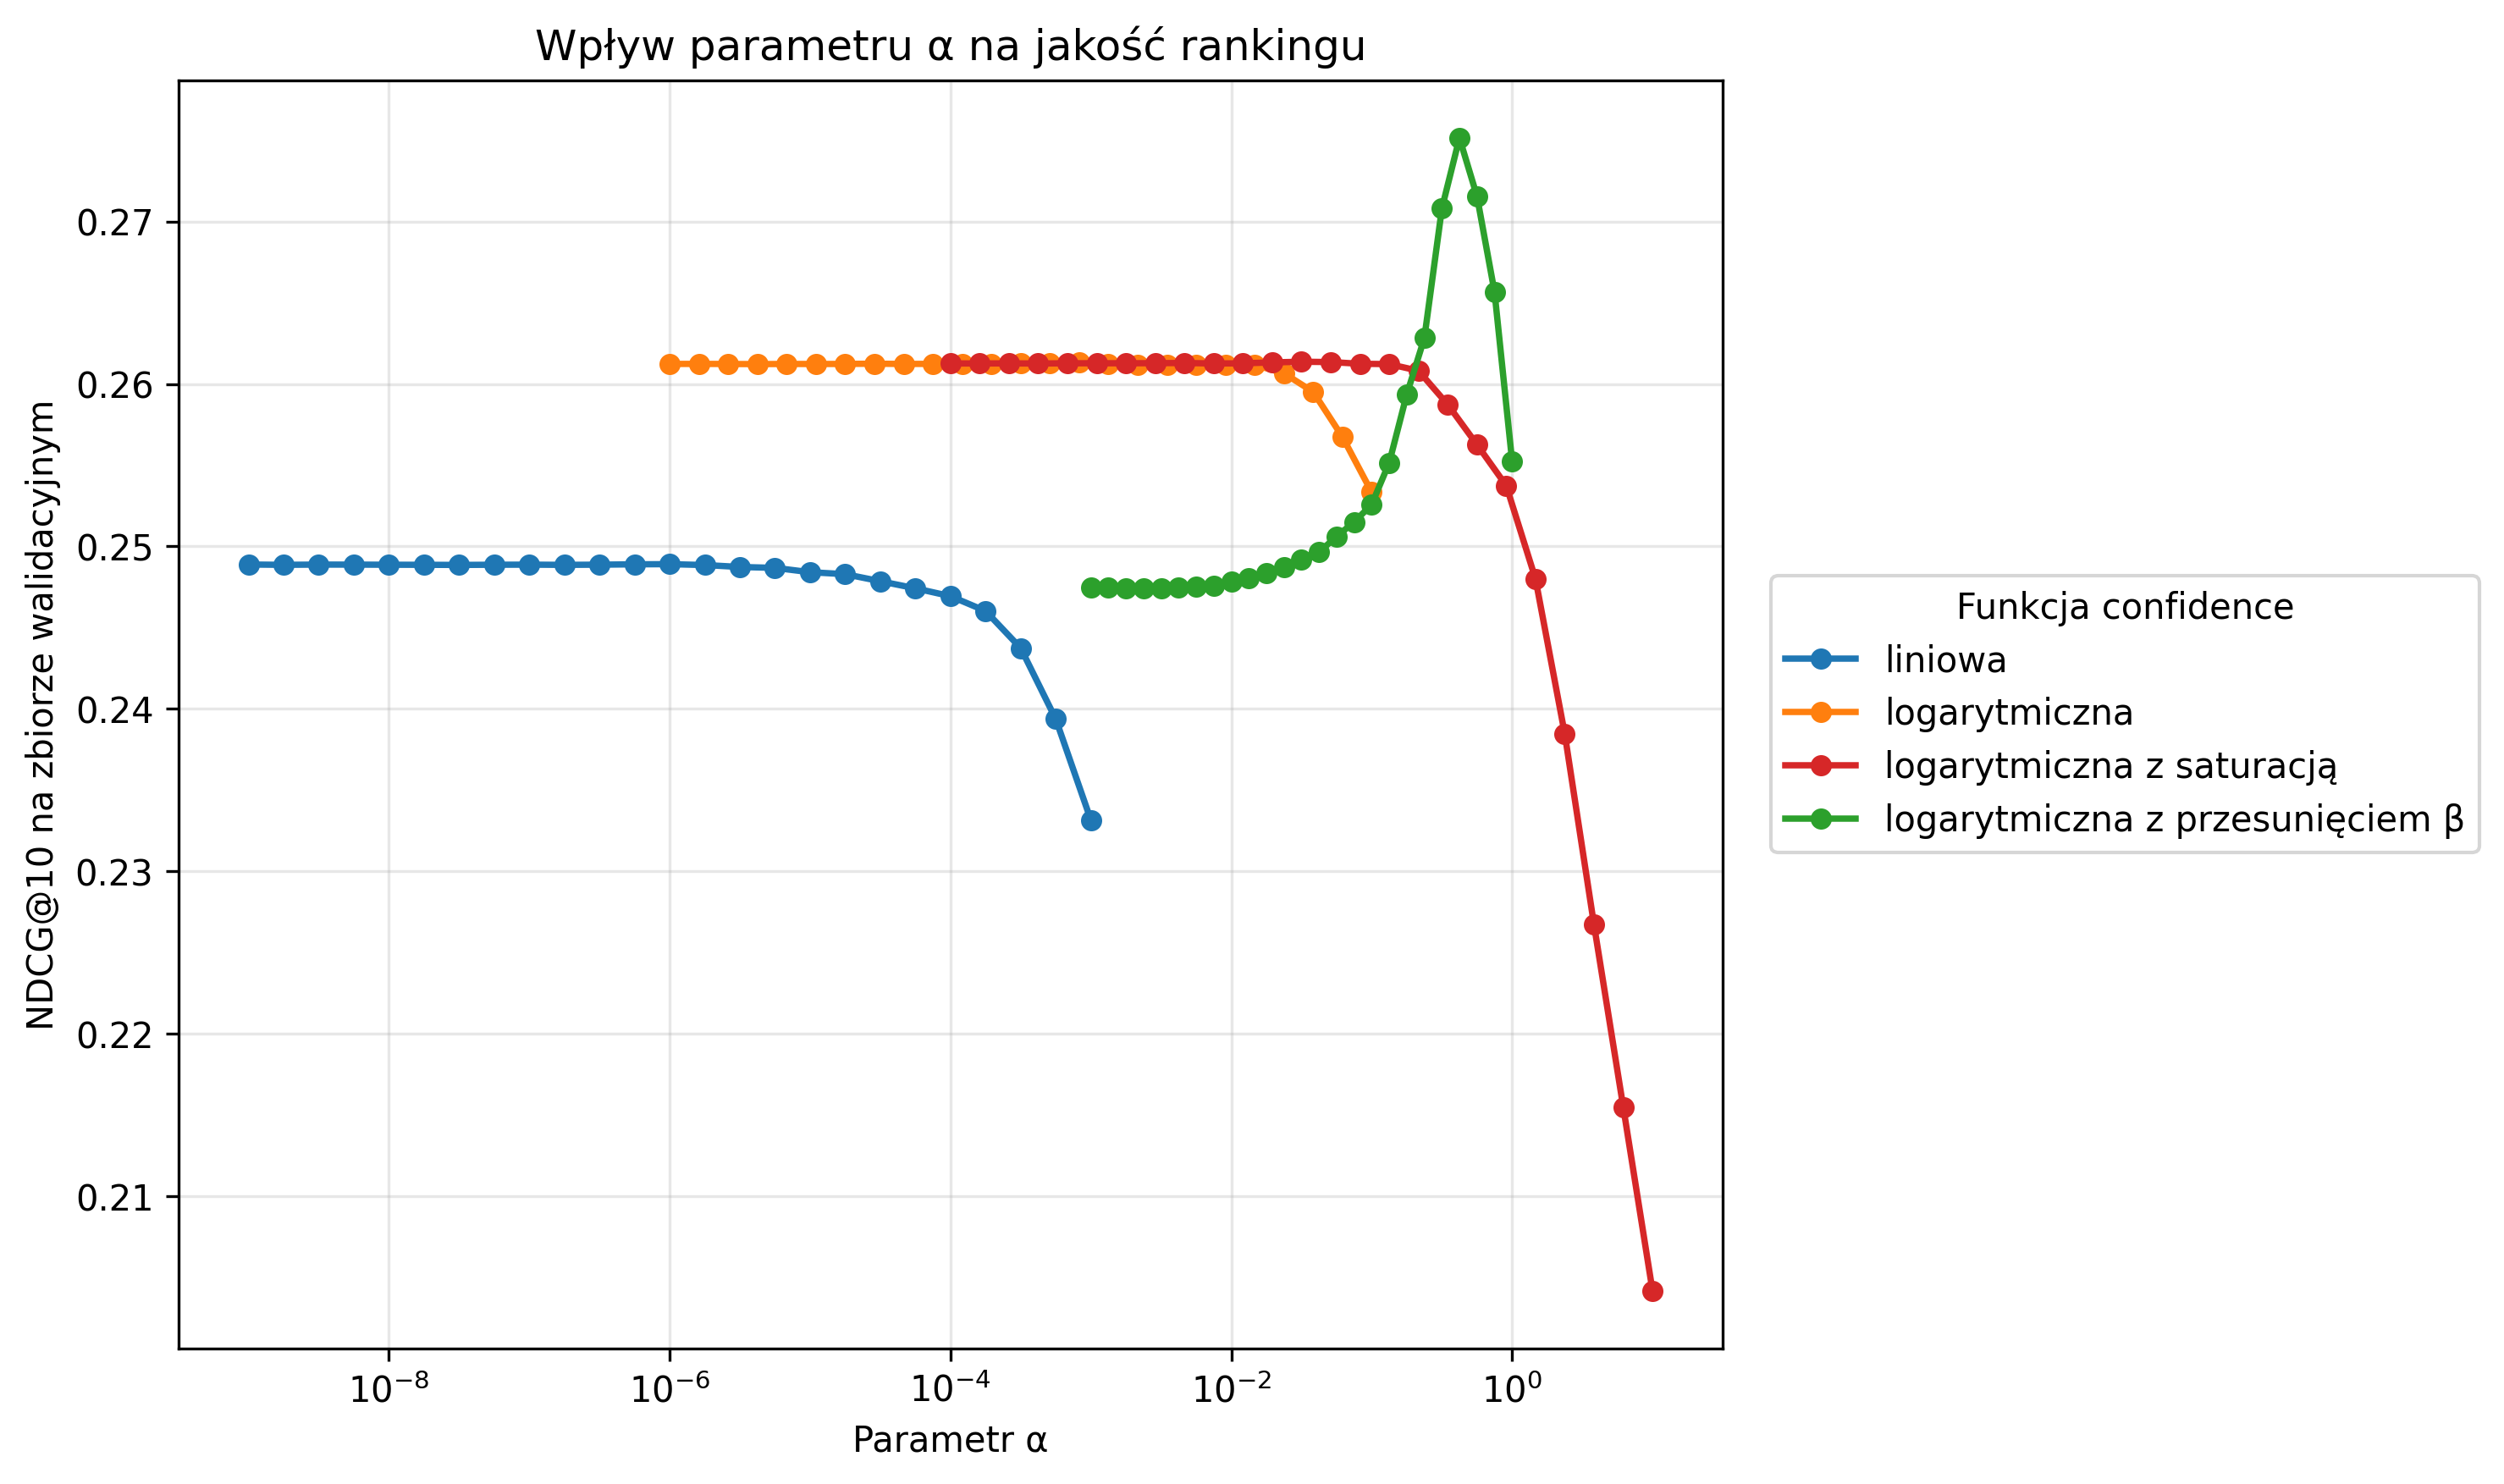
\includegraphics[width=0.9\textwidth]{../results/figures/wrazliwosc_ndcg_vs_alpha.png}
    \caption{Wrażliwość modeli na hiperparametr $\alpha$}
    \label{fig:wrazliwosc_ndcg_vs_alpha}
\end{figure}

Na wykresie~\ref{fig:wrazliwosc_ndcg_vs_alpha} widać, że dla każdej funkcji pewności z wyjątkiem logarytmicznej z przesunięciem $\beta$ wartości \ndcg{} są najwyższe dla $\alpha \rightarrow 0$, co odpowiada zredukowaniu sygnału zawartego w zmiennej \texttt{playtime\_forever} do postaci binarnej, odpowiadającej posiadaniu bądź nieposiadaniu danej gry. W celu zweryfikowania tej obserwacji w kolejnym podrozdziale zostały przebadane funkcje pewności zastosowane w modelach o optymalnych hiperparametrach. Jedynie dla wariantu z dodatkowym przesunięciem $\beta$ znalezione optimum $\alpha$ nie leży w otoczeniu zera. Nie oznacza to jednak, że wariant ten wykorzystuje informację o długości interakcji. Przy $\beta$ równym 108,284 przekształcenie działa w obszarze o niewielkiej krzywiźnie, a wyższa wartość $\alpha$ podnosi przede wszystkim ogólny poziom pewności, nie zaś stopień różnicowania obserwacji. Interpretację tę potwierdza wariant o stałej funkcji pewności, w którym różnicowanie zostało wyeliminowane całkowicie, a mimo to uzyskano najwyższą wartość \ndcg{}.

\begin{figure}[htbp]
    \centering
    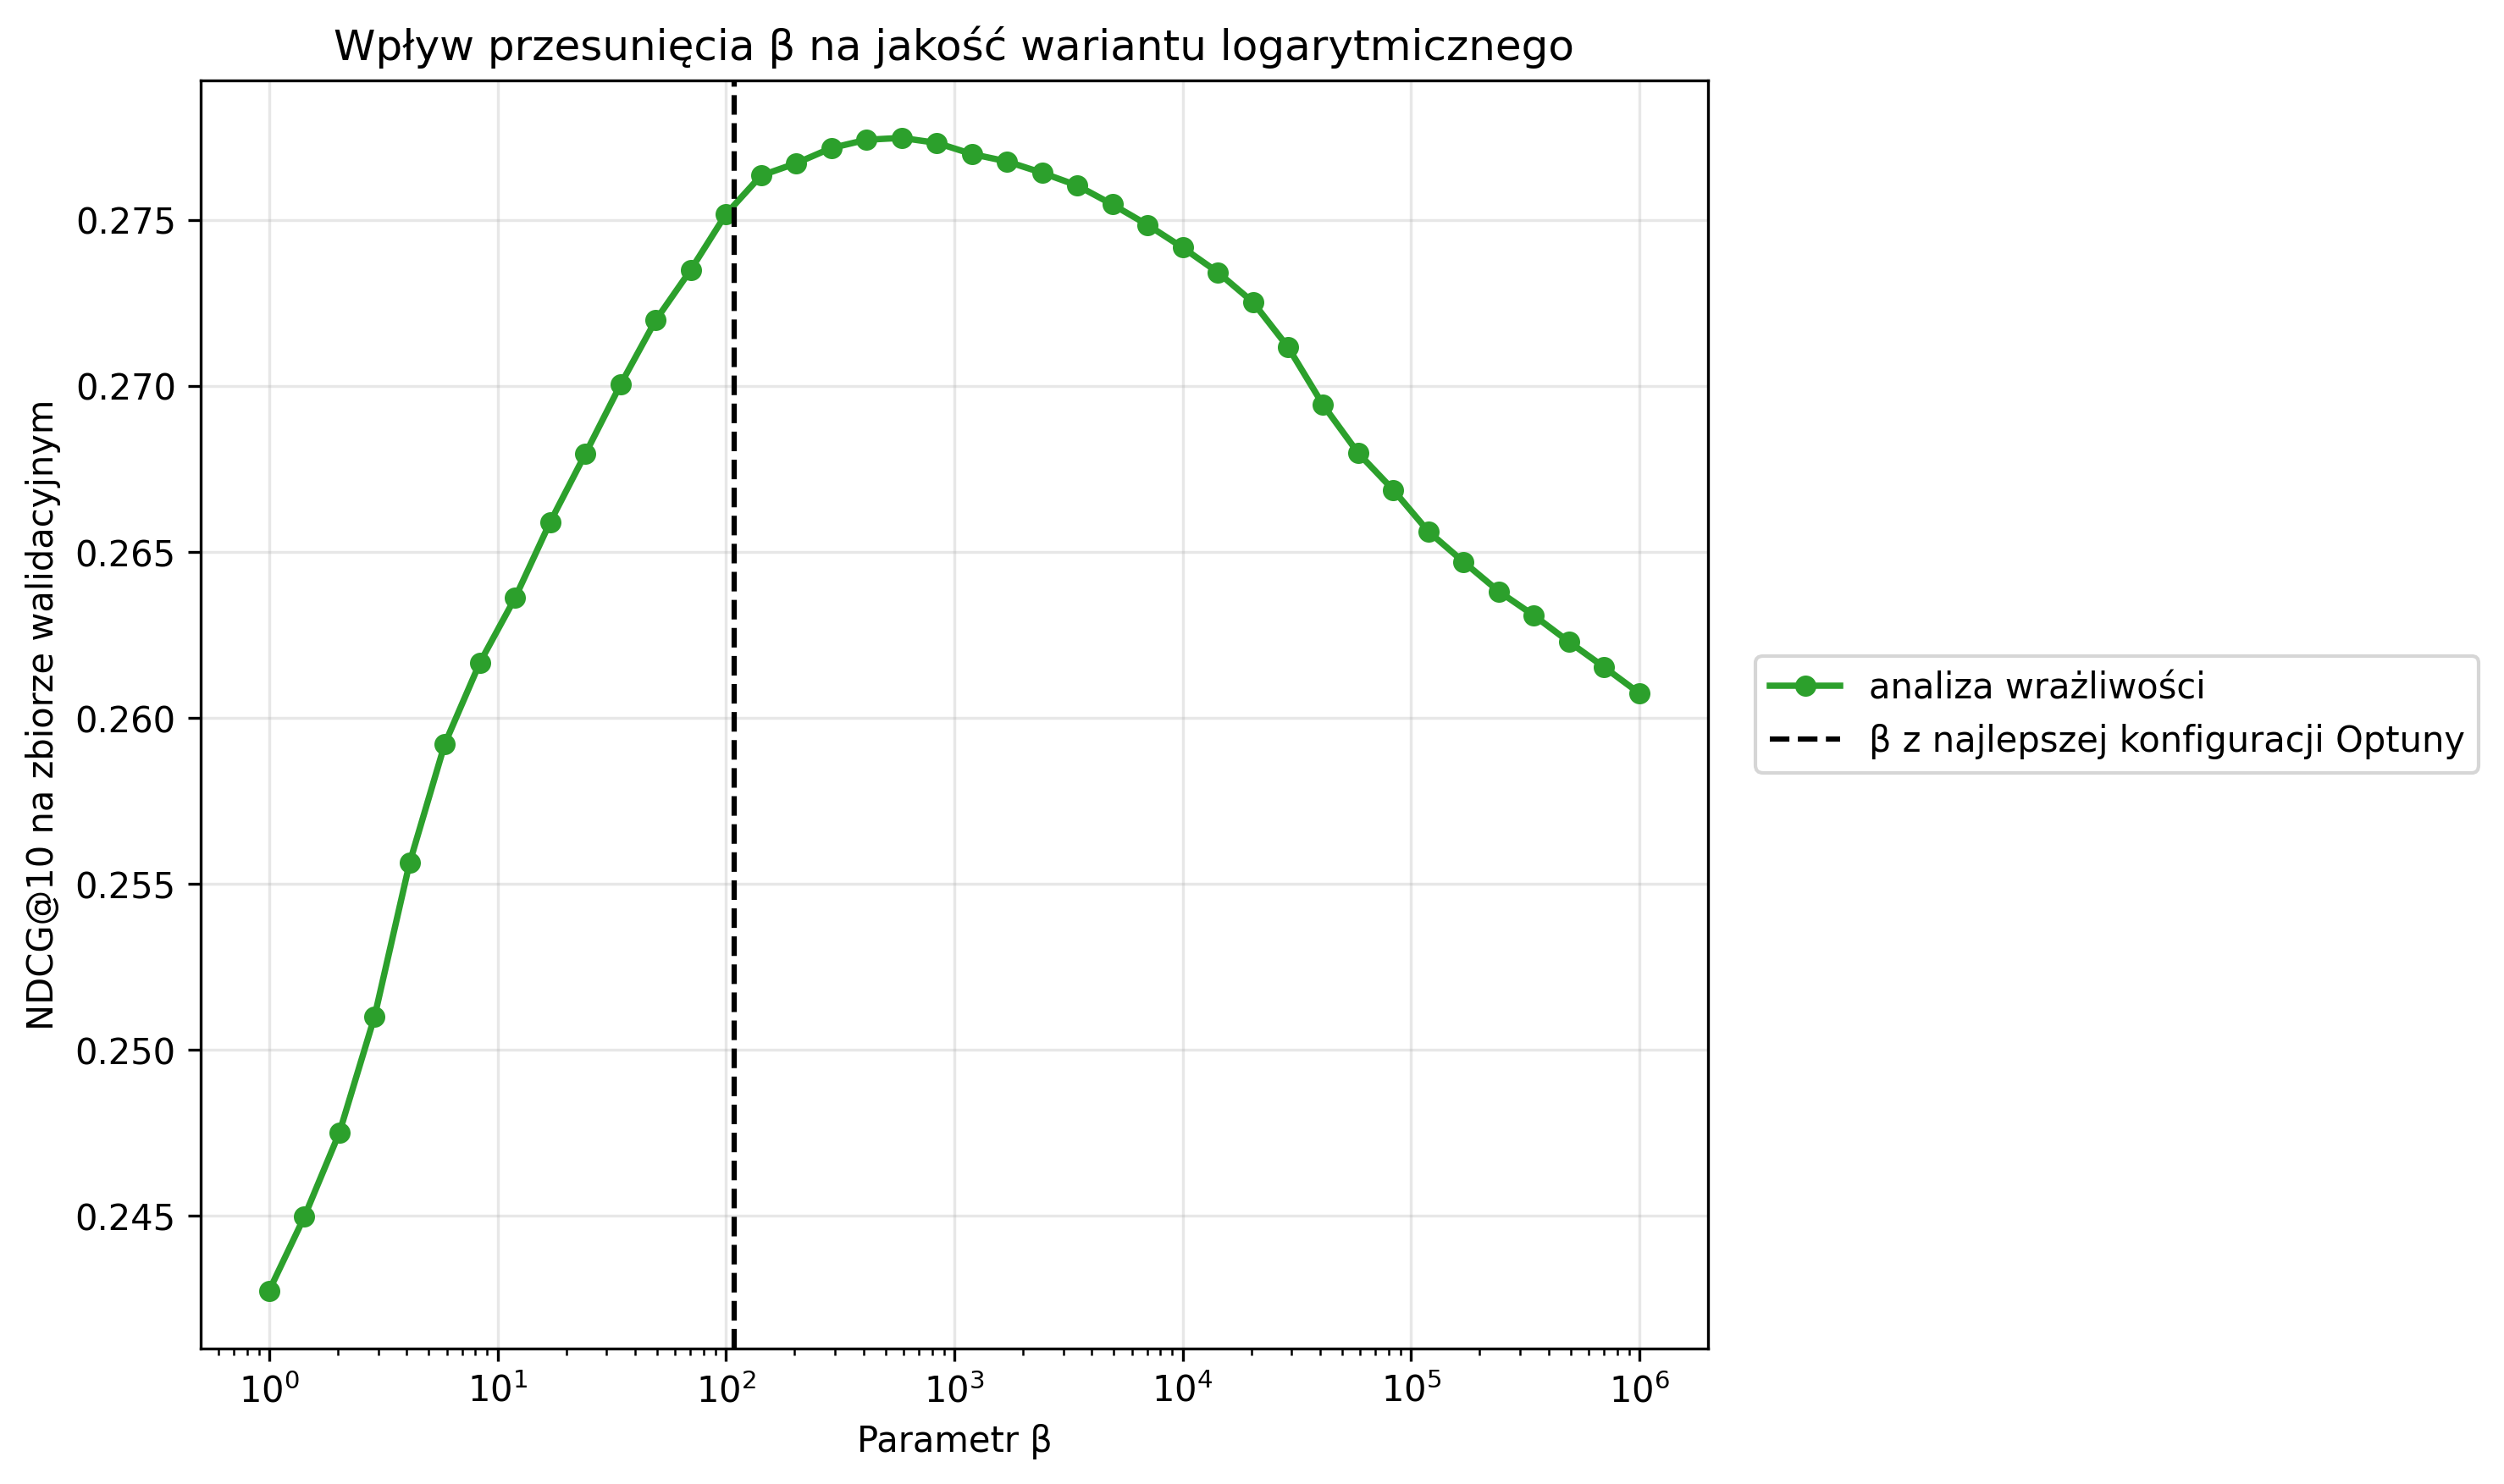
\includegraphics[width=0.9\textwidth]{../results/figures/wrazliwosc_log_beta_ndcg_vs_beta.png}
    \caption{Wrażliwość modelu na hiperparametr $\beta$}
    \label{fig:wrazliwosc_log_beta_ndcg_vs_beta}
\end{figure}

Analogiczną zależność od parametru $\beta$ przedstawiono na wykresie~\ref{fig:wrazliwosc_log_beta_ndcg_vs_beta}. Widać na nim, że wraz ze wzrostem hiperparametru \ndcg{} rośnie, osiągając maksimum dla wartości z rzędu od $10^2$ do $10^4$. Warto podkreślić, że $\beta$ zwiększa wartość $c_{ui}$ obserwacji z \texttt{playtime\_forever} = 0, która w pozostałych modelach zawsze wynosi 1. Dla $\beta$ z otoczenia maksimum mediana wartości pewności rośnie od 1{,}86 przy $\beta$ równym 100 do 3{,}50 przy $\beta$ równym 1000, obejmując tym samym poziom 3{,}364 uzyskany w wariancie o stałej funkcji pewności. Dodatkowo proces strojenia obu modeli doprowadził je do tej samej liczby czynników ukrytych. Warianty różnią się siłą regularyzacji, przy czym obie wartości pozostają w tym samym rzędzie wielkości. Dalsze zwiększanie $\beta$ prowadzi do stopniowego pogorszenia jakości rekomendacji. Wraz z jego wzrostem przekształcenie logarytmiczne dąży do stałej postaci, a średni poziom pewności rośnie. Przez wspólne występowanie obu efektów oraz wpływ regularyzacji na podstawie wyłącznie tego eksperymentu niemożliwe jest stwierdzenie, co dokładnie powoduje spadek jakości. Na wykresie można również zauważyć, że hiperparametry wybrane w procesie strojenia nie są w pełni optymalne, jednak ze względu na marginalność różnic eksperyment był kontynuowany bez ich zmiany.
\begin{figure}[htbp]
    \centering
    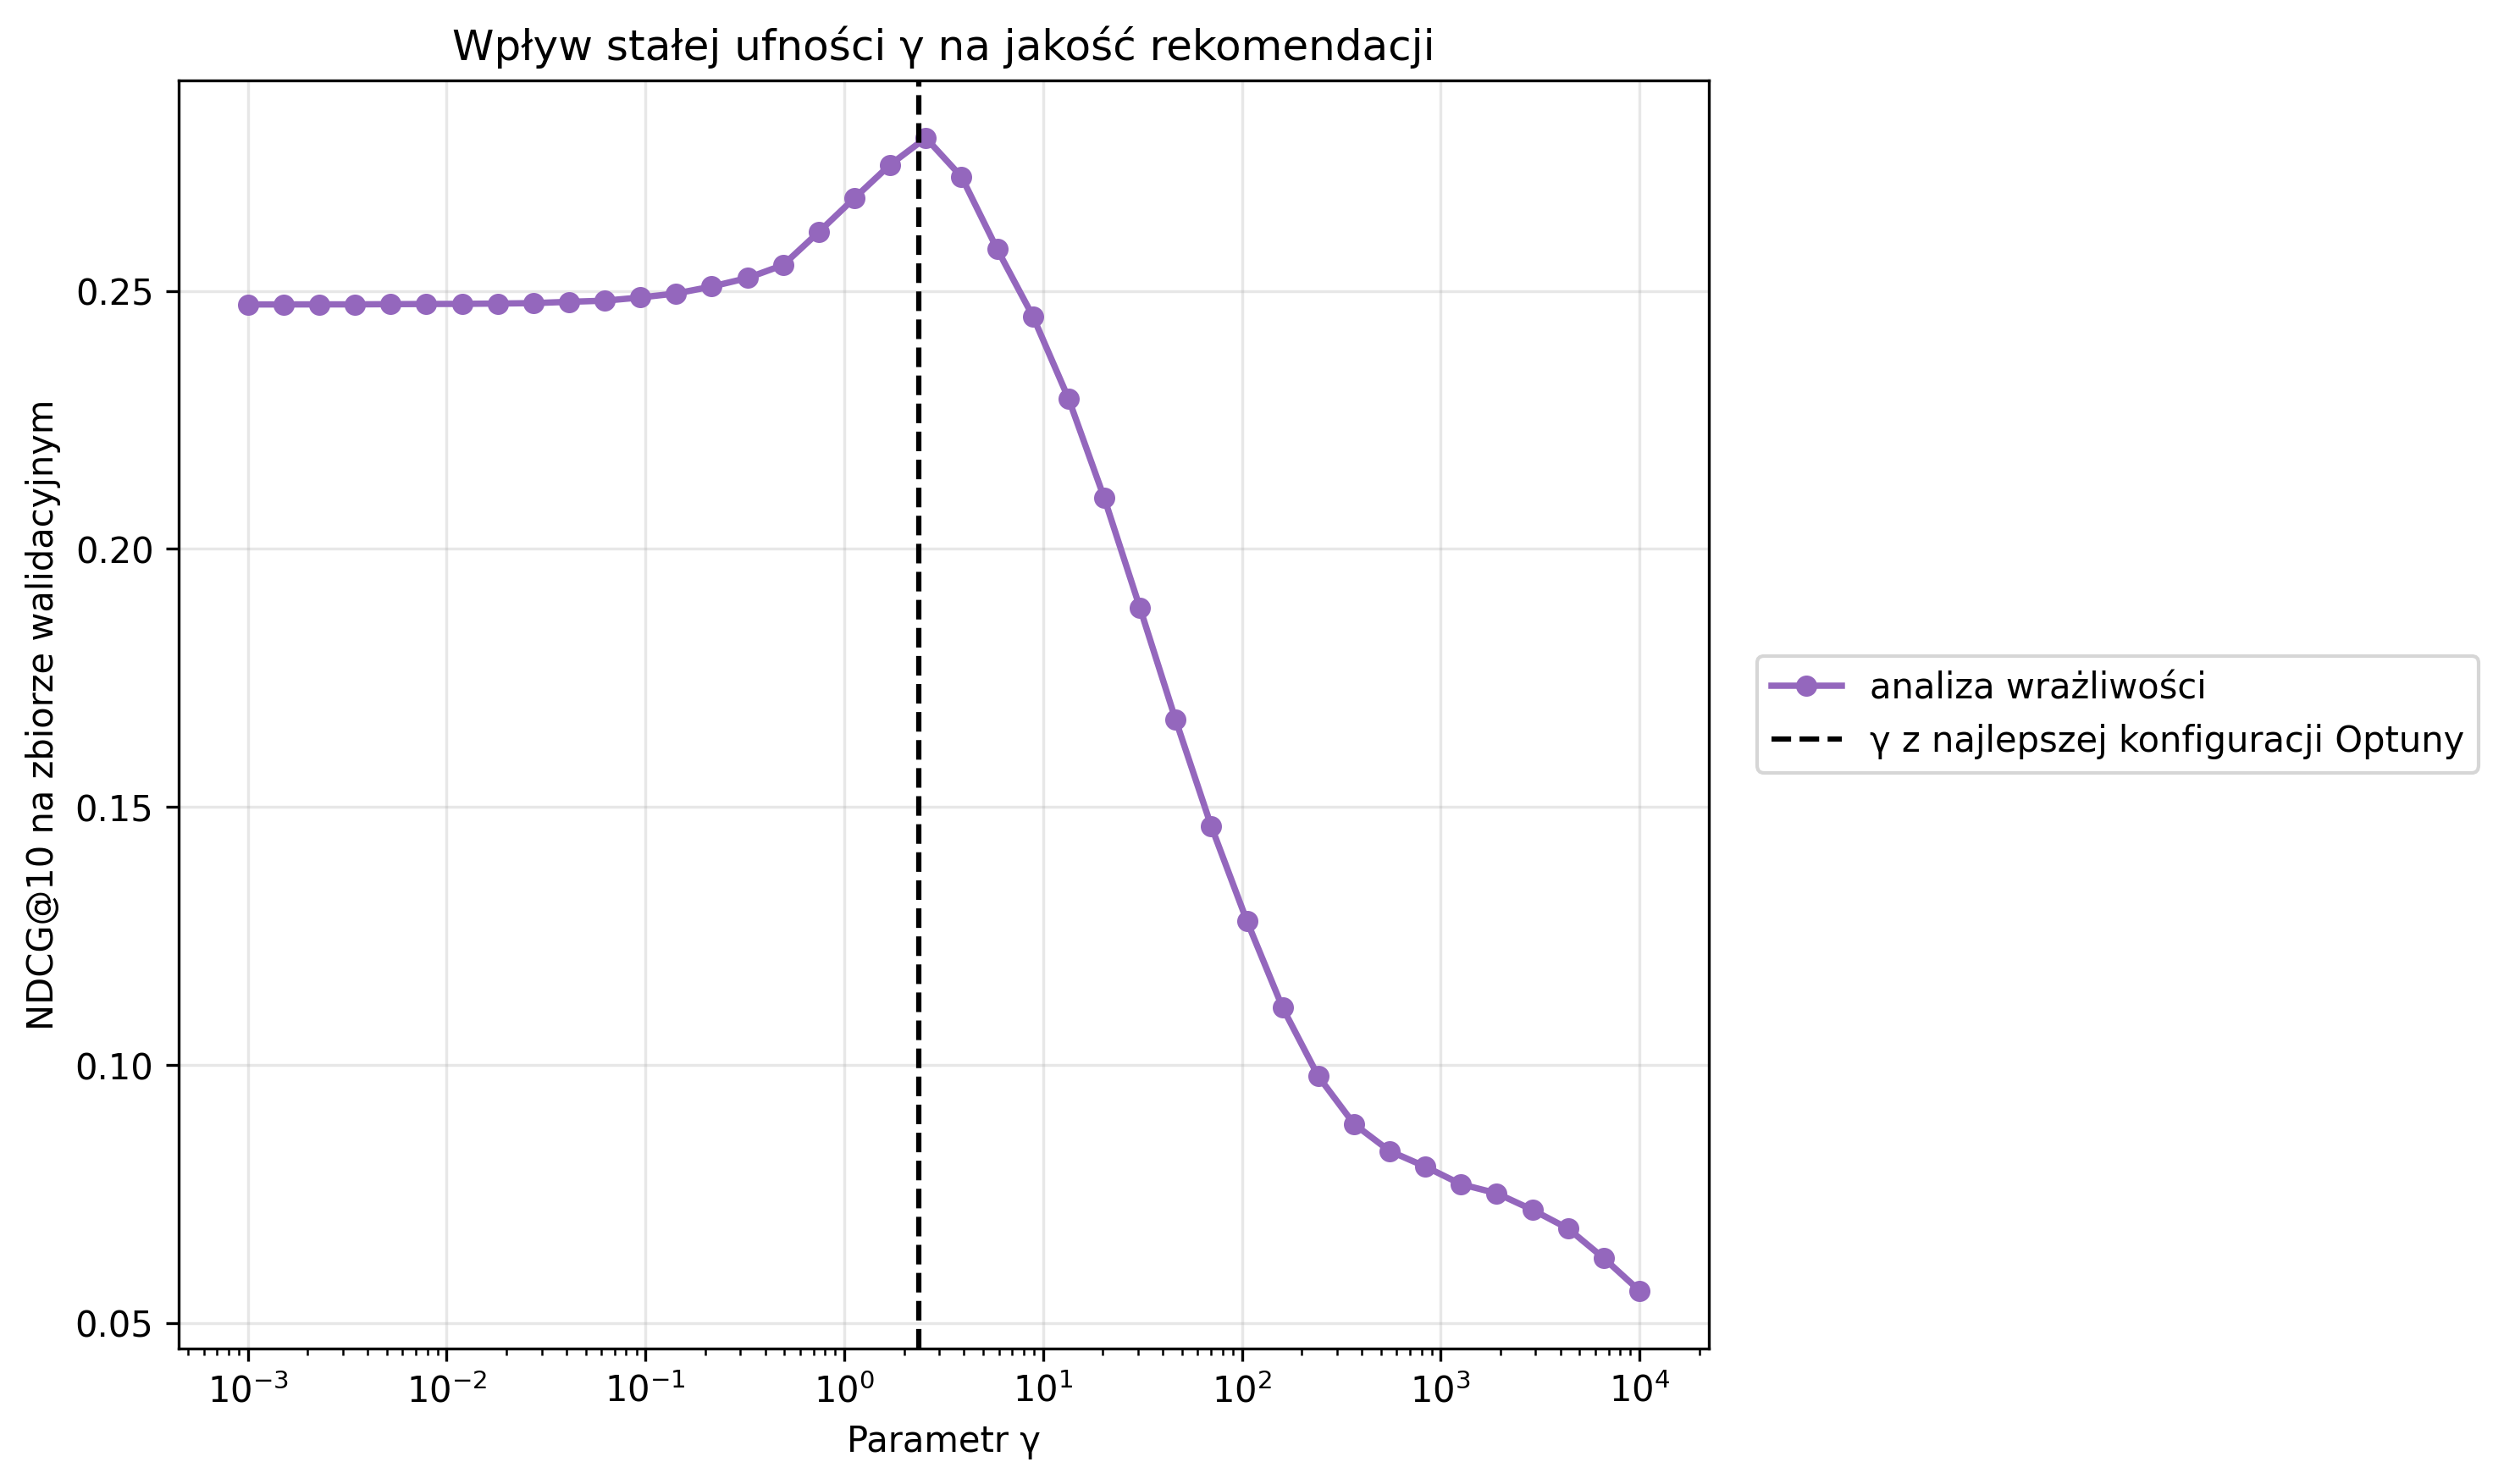
\includegraphics[width=0.9\textwidth]{../results/figures_revised/wrazliwosc_constant_ndcg_vs_gamma.png}
    \caption{Wrażliwość modelu na hiperparametr $\gamma$}
    \label{fig:wrazliwosc_ndcg_vs_gamma}
\end{figure}

Wykres~\ref{fig:wrazliwosc_ndcg_vs_gamma} przedstawia wrażliwość wariantu o stałej funkcji pewności na parametr $\gamma$, wyznaczającego globalny poziom pewności przy całkowitym pominięciu czasu gry. Krzywa ma wyraźne maksimum w okolicy $\gamma$ równego 2{,}5 i opada po obu stronach optimum. Dla $\gamma$ zbliżającego się do zera wartość $c_{ui}$ dąży do jedności, a zatem model traktuje brak interakcji jako równie istotny sygnał jak jej zaobserwowanie. Skutkuje to obniżeniem \ndcg{} do wartości 0{,}247. Dla wartości rzędu $10^4$ jakość rekomendacji drastycznie spada do 0{,}056, ponieważ nadmierna pewność prowadzi do przeuczenia modelu na zaobserwowanych interakcjach. Wynik ten pokazuje, że sam poziom pewności przypisany zaobserwowanym interakcjom istotnie wpływa na jakość rekomendacji, nawet gdy wagi nie różnicują obserwacji w żaden sposób.

Wartości hiperparametrów otrzymane w procesie strojenia modelu BPR zostały przedstawione w tabeli~\ref{tab:hiperparametry-bpr}.

\begin{table}[htbp]
\centering
\caption{Najlepsze hiperparametry modelu BPR wybrane na zbiorze walidacyjnym}
\label{tab:hiperparametry-bpr}
\begin{tabular}{lrrrrr}
\toprule
Wariant & $f$ & $\eta$ & $\lambda_\Theta$ & Iteracje & \ndcg{} \\
\midrule
BPR & $96$ & $0{,}001760$ & $0{,}003237$ & $150$ & $0{,}212$ \\
\bottomrule
\end{tabular}
\caption*{\footnotesize Źródło: opracowanie własne na podstawie wyników optymalizacji hiperparametrów.}
\end{table}


W przypadku modelu BPR nie jest możliwa tak dogłębna analiza dobranych hiperparametrów, ze względu na to, że interakcje traktowane są w sposób binarny. Długość kroku uczenia wpływa wyłącznie na proces wyznaczania maksimum prawdopodobieństwa a posteriori cech ukrytych. Natomiast wymiar przestrzeni cech ukrytych wraz z siłą regularyzacji pozwalają jedynie na oszacowanie złożoności odwzorowywanych relacji oraz swobody, jaką model dysponuje przy tworzeniu wektorów latentnych. Wybrana konfiguracja, obejmująca wyższą liczbę czynników niż w którymkolwiek z wariantów implicit ALS przy stosunkowo niewielkiej regularyzacji, sugeruje lepszą zdolność do tworzenia różnorodnych rekomendacji. Ta kwestia zostanie jednak poddana dalszej analizie w podrozdziale~\ref{sec:compromises_analysis}. 

\section{Analiza funkcji pewności}
\label{sec:confidence_analysis}

Aby zweryfikować hipotezę o redukcji sygnału z \texttt{playtime\_forever} w przypadku modeli implicit ALS przeprowadzono dodatkową analizę funkcji pewności otrzymanych w modelach. Na wykresie~\ref{fig:confidence_levels_best_als} przedstawiono ich zakres wartości dla każdego z modeli.

\begin{figure}[htbp]
    \centering
    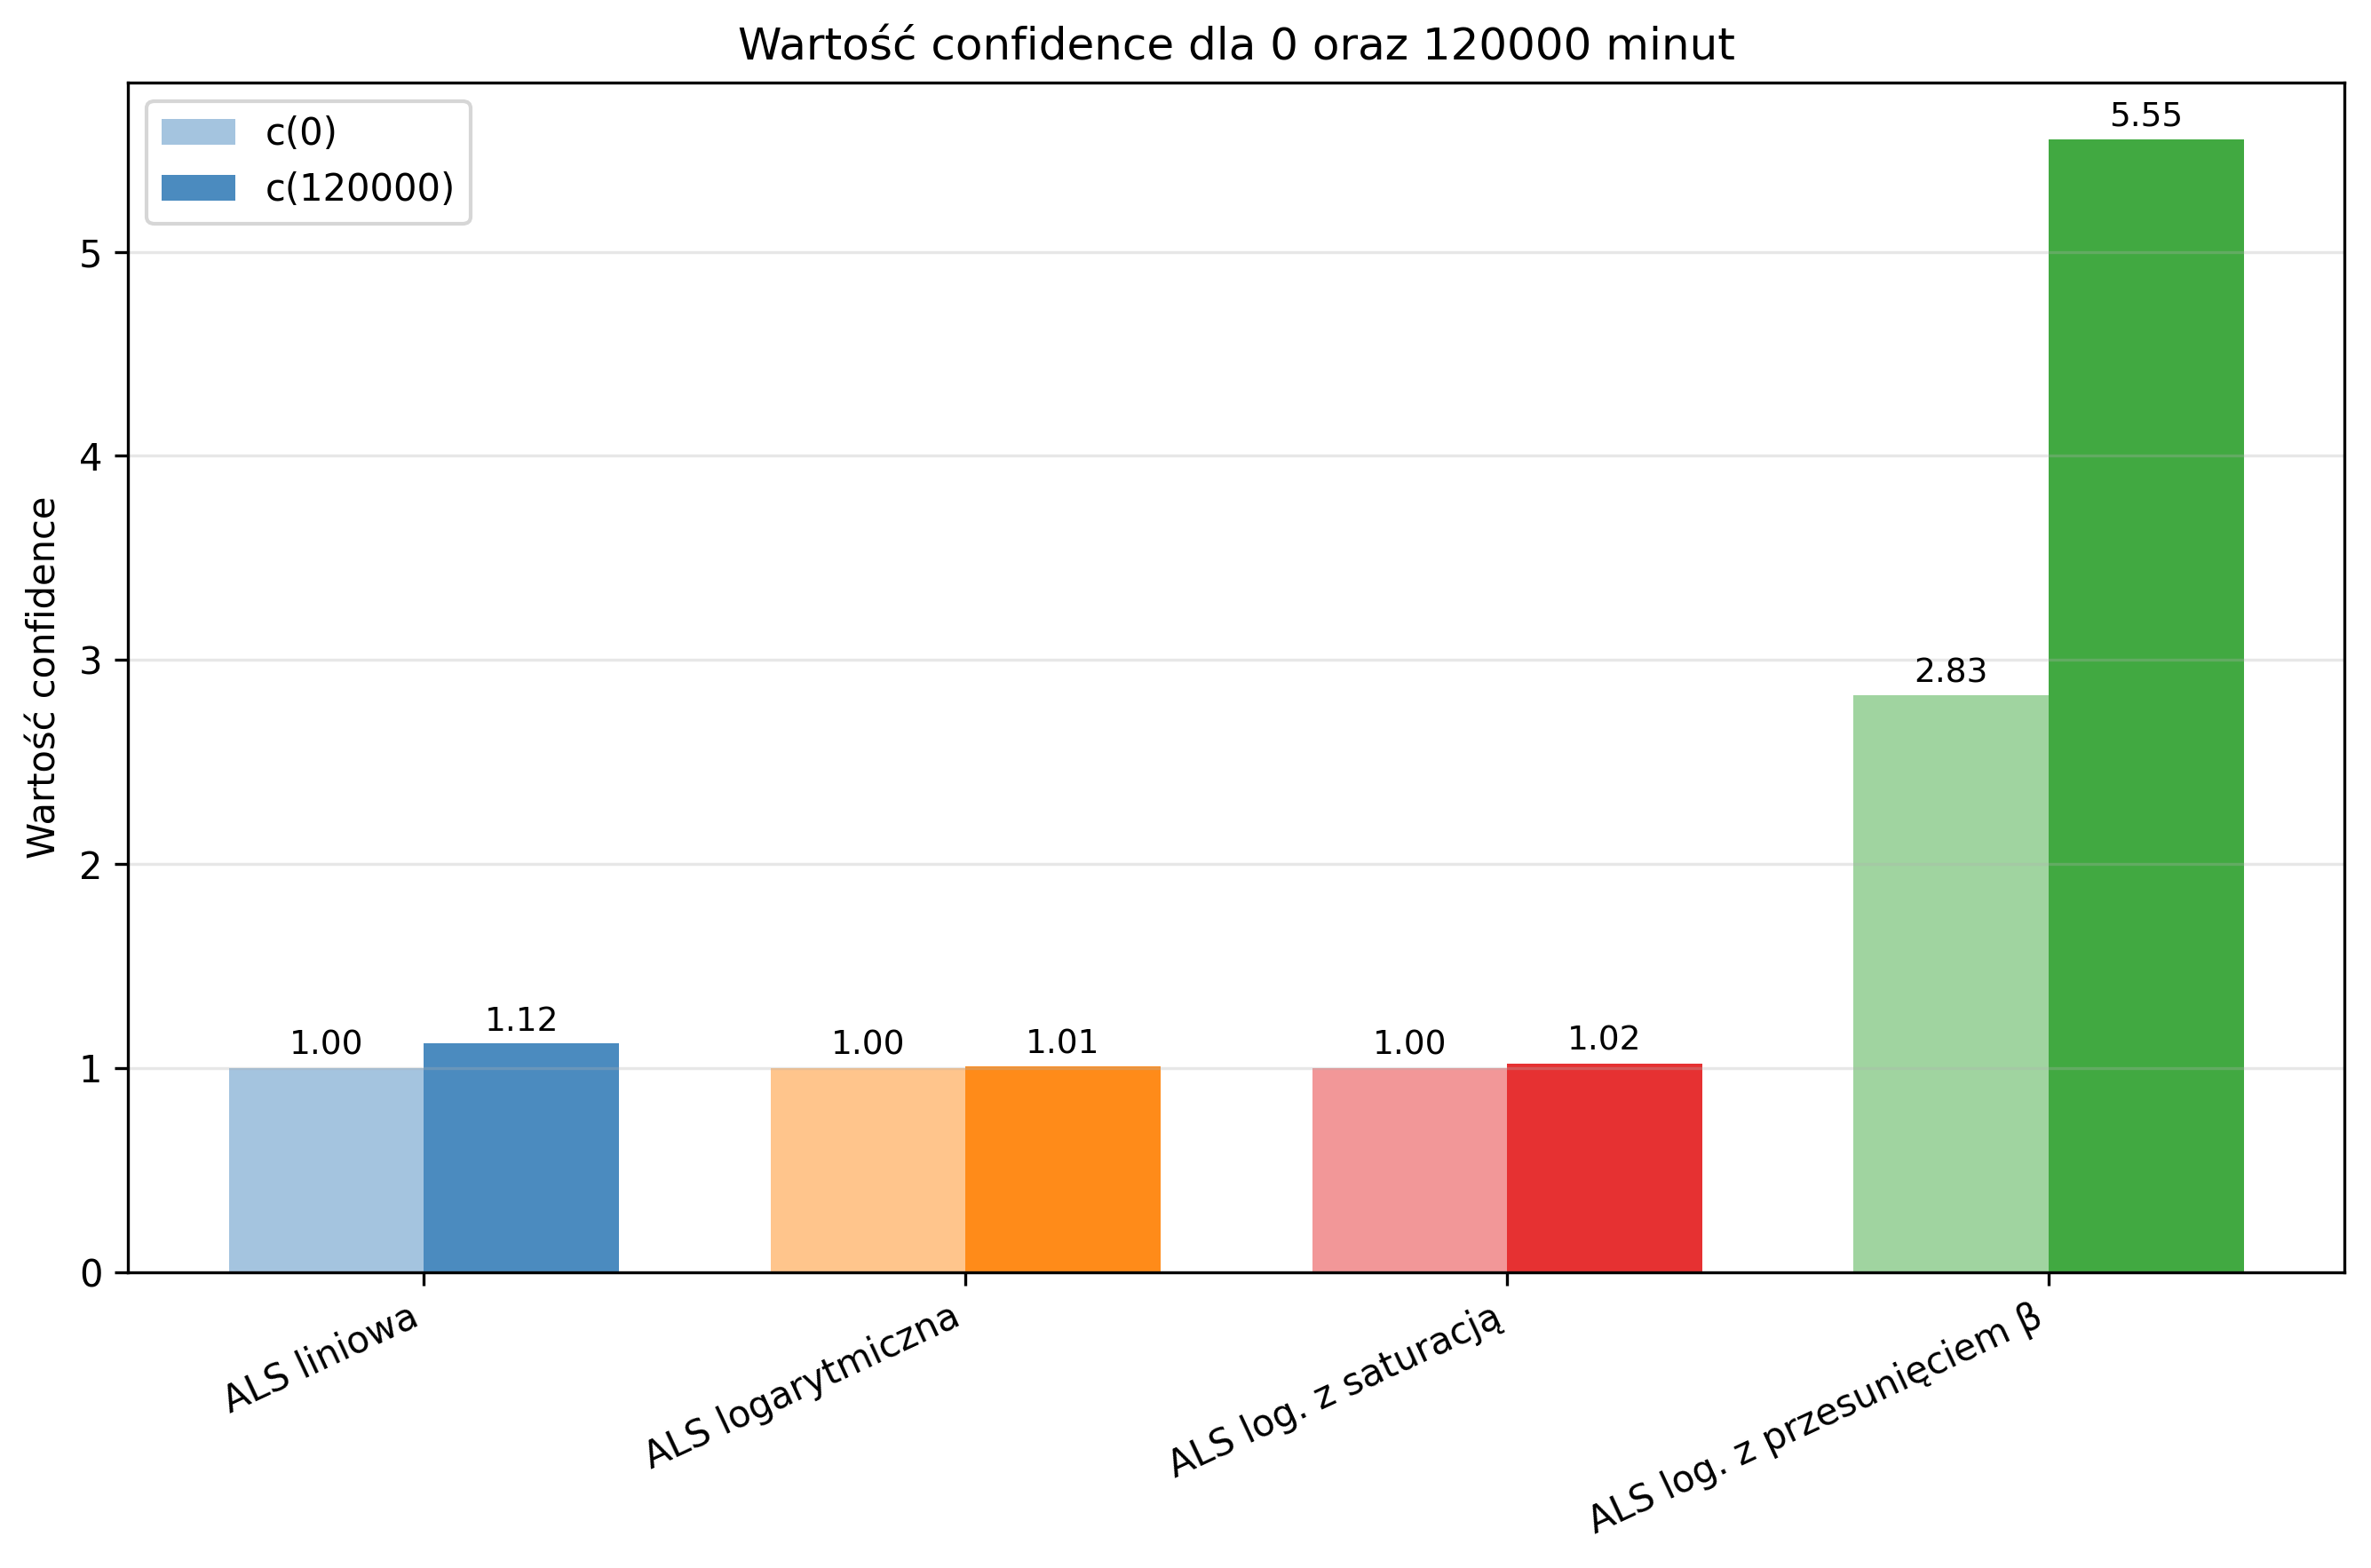
\includegraphics[width=0.9\textwidth]{../results/figures/confidence_levels_best_als.png}
    \caption{Zakres przyjmowanych wartości funkcji pewności}
    \label{fig:confidence_levels_best_als}
\end{figure}

W przypadku modelu z logarytmem oraz logarytmem z saturacją wykres~\ref{fig:confidence_levels_best_als} potwierdza, że długości interakcji mają bardzo znikomy wpływ na proces uczenia. Podobnie w przypadku modelu z liniową funkcją pewności zakresy wartości są niewielkie. Jedynie model z logarytmicznym przekształceniem z przesunięciem $\beta$ po wytrenowaniu uzyskał zakres pewności, który najdłuższym interakcjom przypisuje dwukrotnie większą wartość niż tym bez zarejestrowanego czasu gry.

Zestawienie tego zakresu z wariantem stałym prowadzi jednak do nieoczekiwanego wniosku. Przesunięcie $\beta$ podnosi dolną granicę zakresu funkcji odpowiadającą obserwacjom z zerowym czasem gry z wartości równej 1 do poziomu 2,83. Dla mediany czasu gry wynoszącej 35 minut wartość ta rośnie zaledwie do 2,94, pozostając w tym samym rzędzie co stała wartość 3,364 dobrana w wariancie pomijającym czas gry. Zatem dla znacznej części zbioru przekształcenie działa w wąskim przedziale wokół poziomu, który sam w sobie okazuje się wystarczający do uzyskania lepszych rekomendacji, a zróżnicowanie wag ujawnia się dopiero dla obserwacji z długiego ogona rozkładu.

Należy jednak podkreślić, że w procesie optymalizacji modelu implicit ALS uwzględniane są wszystkie możliwe kombinacje par użytkownik--gra, a przy gęstości macierzy interakcji wynoszącej 0,00887 przypadki niezaobserwowane, dla których $c_{ui} = 1$, zdecydowanie dominują w funkcji celu. Zmiana wartości $c_{ui}$ dla nielicznych interakcji pozytywnych oddziałuje więc przede wszystkim przez ogólne podniesienie ich wagi względem tła, w mniejszym stopniu zaś przez wzajemne różnicowanie tych obserwacji. Wskazuje to, że przewaga wariantu z przesunięciem $\beta$ nad pozostałymi przekształceniami wynikała nie tyle z lepszego odwzorowania siły preferencji, ile z podniesienia pewności wszystkich zaobserwowanych interakcji, w tym tych z zerowym czasem gry. Wariant o stałej funkcji pewności realizuje ten sam mechanizm, bez przekształcenia czasu gry osiągając podobne rezultaty.

Aby przyjrzeć się bliżej kształtowi poszczególnych przekształceń, stworzono wykres~\ref{fig:confidence_growth_best_als_0_2400} przedstawiający przyrost wartości funkcji pewności w modelach implicit ALS w zależności od zmiennej \texttt{playtime\_forever} dla pierwszych 20 godzin rozgrywki.

\begin{figure}[htbp]
    \centering
    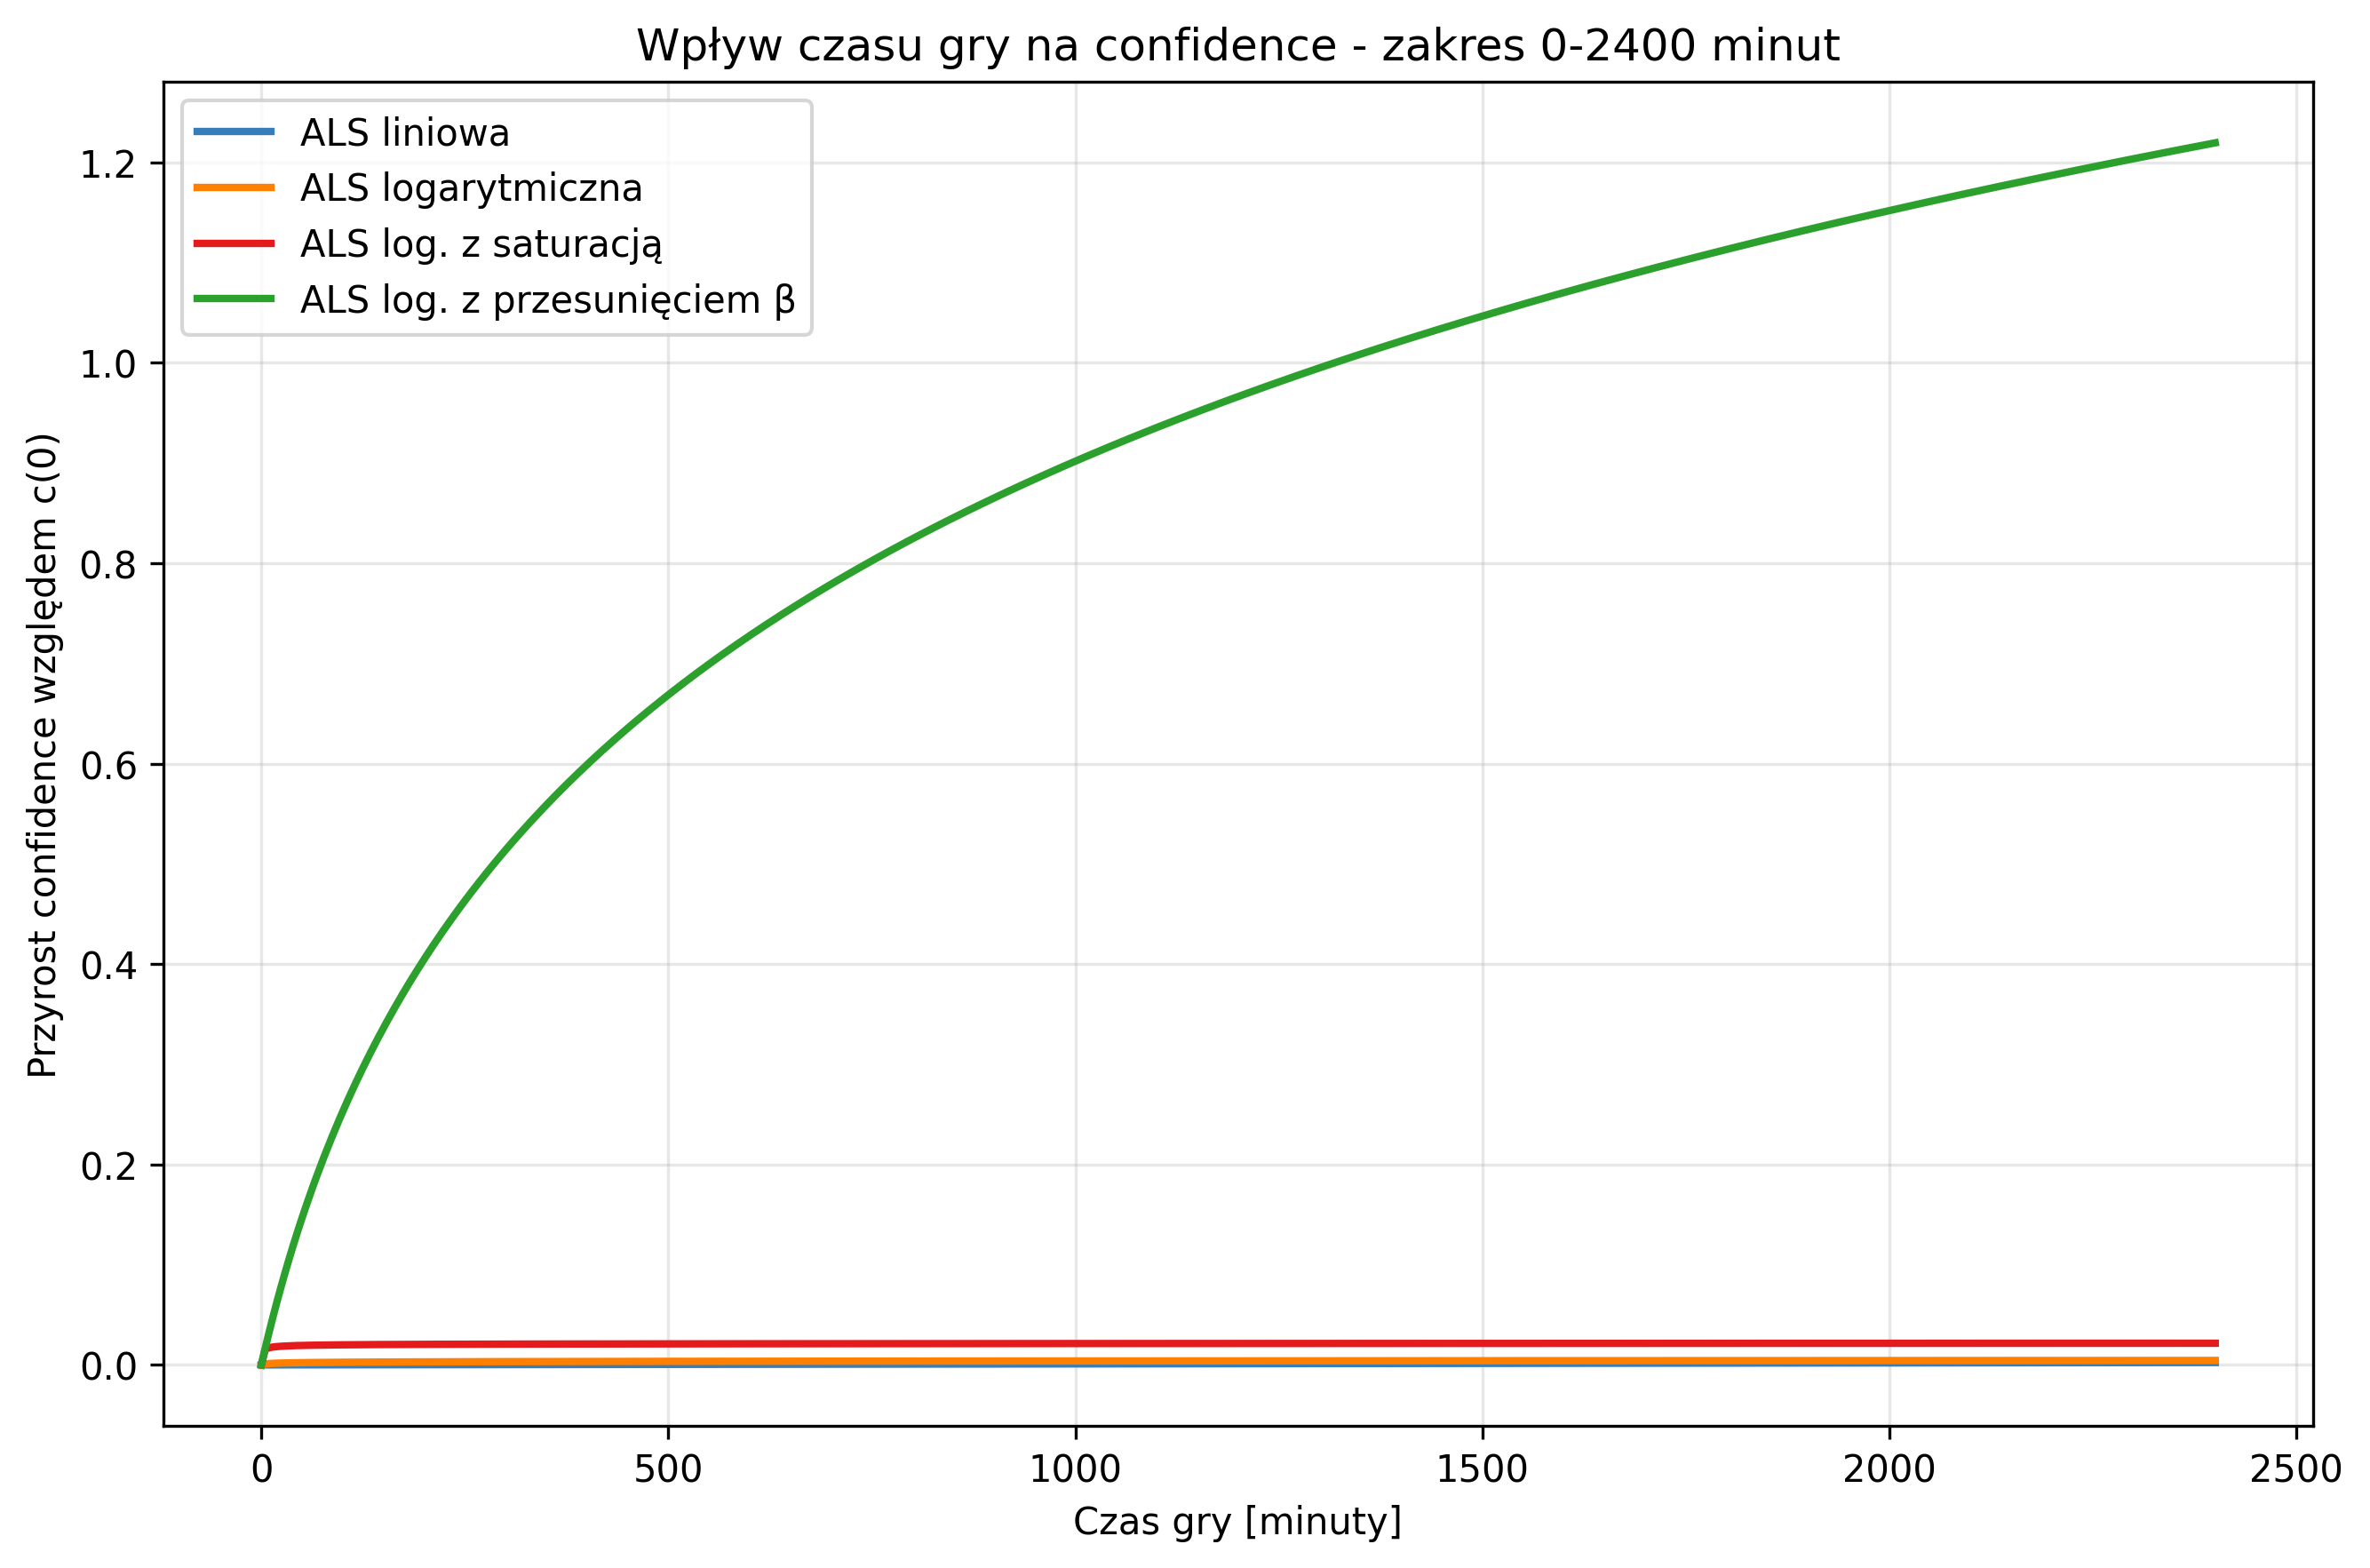
\includegraphics[width=0.9\textwidth]{../results/figures/confidence_growth_best_als_0_2400.png}
    \caption{Wartości pewności w zależności od zmiennej \texttt{playtime\_forever}}
    \label{fig:confidence_growth_best_als_0_2400}
\end{figure}

% ten wykres moze powinien byc nie przyrostem a po prostu wartoscią
% może też powinien być na całej skali od 0 do 120000

Przebieg krzywych na wykresie~\ref{fig:confidence_growth_best_als_0_2400} obrazuje różnicę między wariantem z przesunięciem $\beta$ a pozostałymi przekształceniami. Podczas gdy dla pozostałych modeli funkcja przyrostu wartości pewności pozostaje bliska 0, model z $c_{ui} = 1 + \alpha\log(1 + r_{ui} + \beta)$ wykazuje wyraźny wzrost. W przedziale pierwszych kilkuset minut rozgrywki przyrost wartości $c_{ui}$ jest stosunkowo szybki, natomiast w dalszej części wykresu krzywa widocznie łagodnieje. Należy jednak zestawić skalę tego przyrostu z poziomem bazowym. Dla mediany czasu gry przyrost względem $c(0)$ wynosi zaledwie 0,11 przy wartości bazowej 2,83. Widoczna na wykresie zmienność dotyczy zatem przede wszystkim mniejszościowej części zbioru, a dla typowego użytkownika funkcja pozostaje w wąskim otoczeniu wartości stałej.

Warto rozważyć teoretyczny przyrost pozostałych wariantów transformacji w przypadku, gdyby nie uległy one skrajnemu spłaszczeniu. Dla modelu z $c_{ui} = 1 + \alpha \log(r_{ui} + 1)$ dla domyślnego hiperparametru $\alpha = 1$ zaledwie 19 minut rozgrywki wystarczy, aby wartość pewności modelu gwałtownie skoczyła od poziomu bazowego równego 1 aż do 4. Równocześnie, aby uzyskać wzrost z poziomu 7 do 8, użytkownik musi spędzić w grze w przybliżeniu dodatkowe 11 i pół godziny. Oznacza to, że ta funkcja wykazuje się znaczną czułością w wąskim przedziale małych wartości, podczas gdy zmiana wśród dużych wartości jest nieznaczna. Podobny efekt obserwuje się w przypadku funkcji
$c_{ui} = 1 + \alpha \frac{\log(1 + r_{ui})}{1 + \log(1 + r_{ui})}$. Natomiast w przypadku liniowej funkcji pewności $c_{ui} = 1 + \alpha r_{ui}$ to zjawisko przybiera odwrotny charakter. Ponieważ jej przyrost jest proporcjonalny do spędzonego czasu, model nie posiada efektu saturacji. W efekcie użytkownicy generujący skrajnie wysokie liczby godzin uzyskiwaliby dominujący wpływ na wartość funkcji straty. Proces optymalizacji hiperparametrów przeciwdziała temu, dobierając $\alpha$ rzędu $10^{-6}$, co w praktyce sprowadza przekształcenie do postaci niemal stałej. Zarówno w tym przypadku, jak i dla wariantów logarytmicznych, optymalizacja konsekwentnie zmierza zatem w stronę ograniczenia zróżnicowania wag, niezależnie od kształtu samego przekształcenia.

\section{Jakość rekomendacji na zbiorze testowym}

Przedstawione różnice w procesie uczenia mają swoje odzwierciedlenie w metrykach otrzymanych na zbiorze testowym. W tabeli~\ref{tab:wyniki-glowne} przedstawiono uśrednione wyniki otrzymane dla każdego z modeli. Dla zachowania czytelności w~tabeli pominięto odchylenia standardowe;
przedstawiono je w~podrozdziale~\ref{sec:stabilnosc}.

\begin{table}[htbp]
\centering
\caption{Wyniki modeli na zbiorze testowym}
\label{tab:wyniki-glowne}
\resizebox{\textwidth}{!}{%
\begin{tabular}{lrrrrrr}
\toprule
Model & NDCG@10 & Precision@10 & Recall@10 & Coverage@10 & $\Delta$GAP@10 & ILD@10\\
\midrule
Popularność & $0{,}1855$ & $0{,}0965$ & $0{,}1783$ & $0{,}0087$ & $1{,}4233$ & --- \\
ALS liniowa & $0{,}3299$ & $0{,}1841$ & $0{,}2642$ & $0{,}1178$ & $-0{,}2112$ & $0{,}7528$ \\
ALS logarytmiczna & $0{,}3356$ & $0{,}1810$ & $0{,}3019$ & $0{,}0762$ & $0{,}5433$ & $0{,}6469$ \\
ALS log. z saturacją & $0{,}3354$ & $0{,}1809$ & $0{,}3019$ & $0{,}0761$ & $0{,}5443$ & $0{,}6470$ \\
ALS log. z przesunięciem $\beta$ & $0{,}3517$ & $0{,}1956$ & $0{,}3338$ & $0{,}1313$ & $0{,}4191$ & $0{,}6841$ \\
ALS stała & $\mathbf{0{,}3565}$ & $\mathbf{0{,}1978}$ & $\mathbf{0{,}3370}$ & $0{,}1374$ & $0{,}4210$ & $0{,}6825$ \\
BPR & $0{,}2703$ & $0{,}1329$ & $0{,}2614$ & $\mathbf{0{,}3039}$ & $-0{,}0789$ & $0{,}7363$ \\
\bottomrule
\end{tabular}%
}
\caption*{\footnotesize Źródło: opracowanie własne. Wartości dla ALS i BPR to średnie z~pięciu uruchomień, z~wyjątkiem ILD@10, wyznaczonej dla pojedynczego uruchomienia. Pogrubieniem oznaczono najlepszy wynik w~każdej kolumnie.}
\end{table}

Ze względu na dużą liczbę metryk w tym podrozdziale skupiono się na metrykach rankingowych, pozostałe z nich zostaną przeanalizowane w kolejnym podrozdziale poświęconym kompromisom między nimi. Ze względu na stosowanie metryki \ndcg{} jako głównej metryki rankingowej w celu lepszego zaprezentowania różnic między modelami utworzono wykres~\ref{fig:test_ndcg_all_models_horizontal}, który przedstawia jej wartość dla każdego z testowanych modeli.

\begin{figure}[htbp]
    \centering
    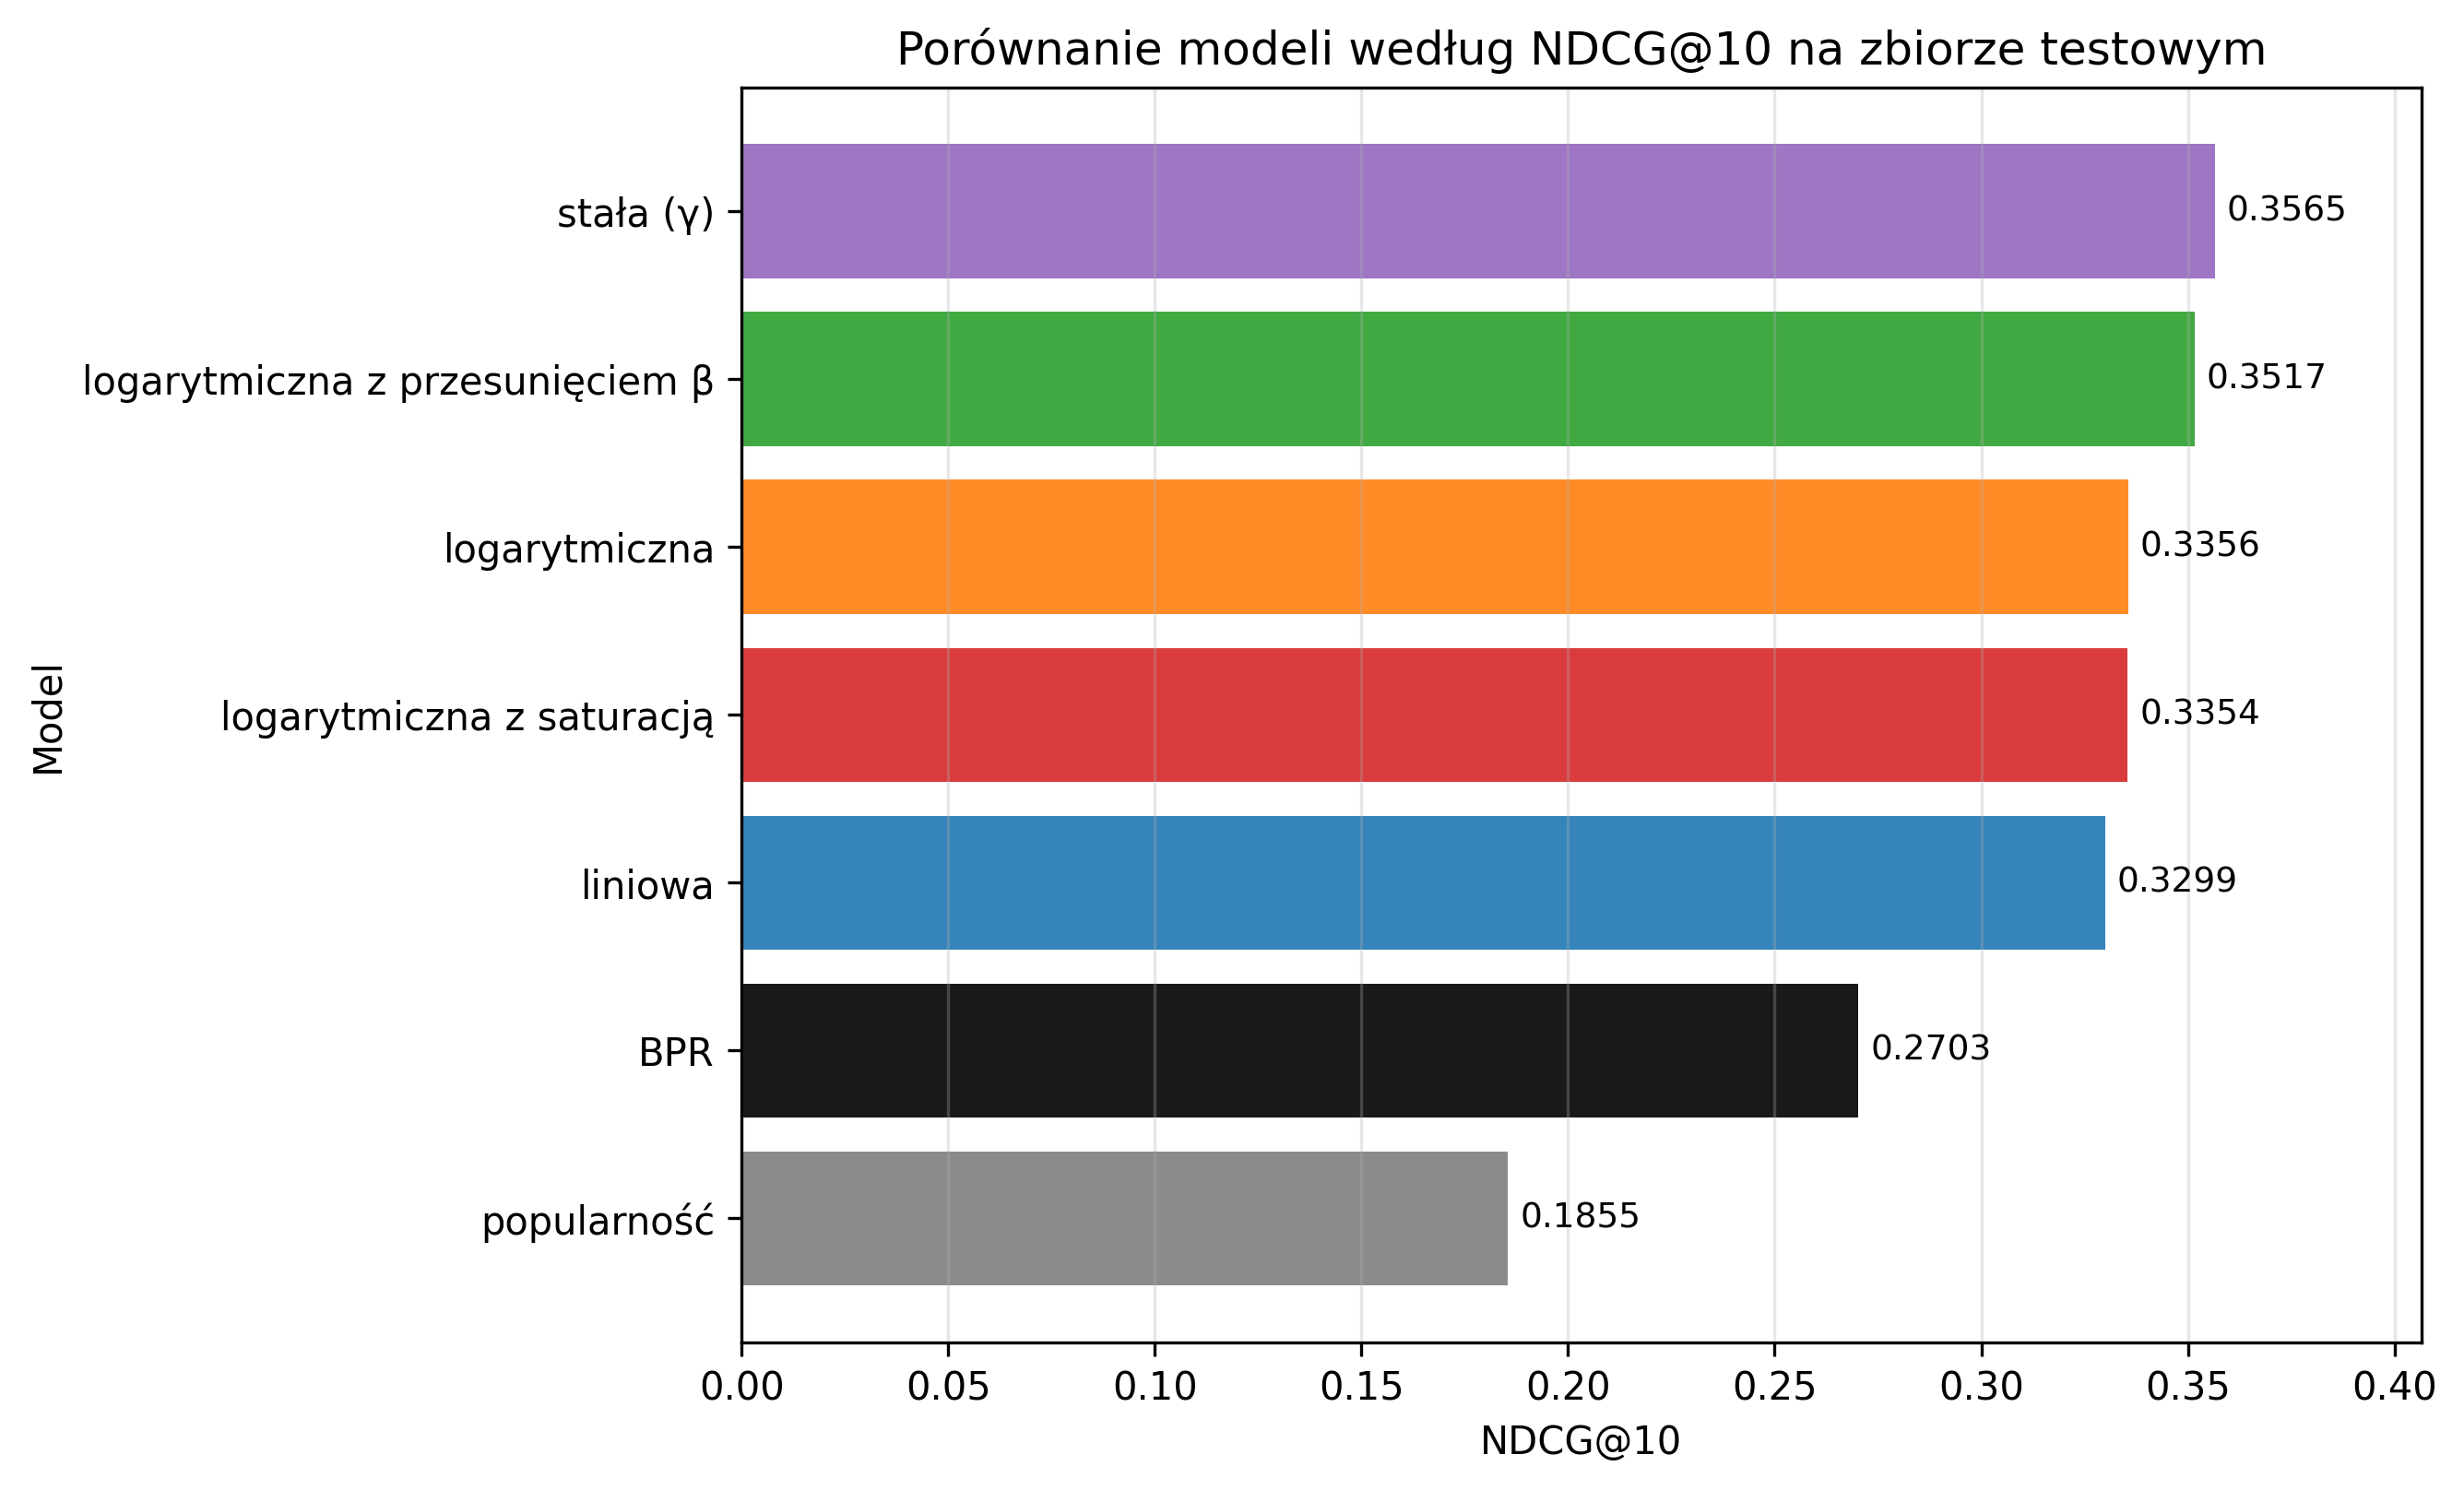
\includegraphics[width=0.9\textwidth]{../results/figures_revised/test_ndcg_all_models_horizontal.png}
    \caption{Wartości \ndcg{} każdego z modeli na zbiorze testowym}
    \label{fig:test_ndcg_all_models_horizontal}
\end{figure}

Wykres jednoznacznie pokazuje, że model popularnościowy cechuje się niższą zdolnością rekomendacji niż modele oparte na metodach faktoryzacji macierzy. Mimo to uzyskany wynik nie jest zaniedbywalny. Model popularnościowy efektywnie wykorzystuje silny efekt nierównomierności popularności gier w analizowanym zbiorze danych przedstawiony na wykresie~\ref{fig:filtered_item_popularity_concentration}. Ze względu na to został on wykorzystany jako punkt odniesienia w niniejszej pracy.

Uzyskana przez BPR wartość \ndcg{} jest najniższa spośród wszystkich modeli faktoryzacji. Należy jednak podkreślić, że nie oznacza to, że model jest obiektywnie gorszy. W ocenie systemów rekomendacyjnych należy również uwzględniać metryki odpowiedzialne za pokrycie katalogu i podatność na obciążenie popularnością.

Istotnych wniosków dostarcza porównanie poszczególnych wariantów modelu ALS między sobą. Najwyższą wartość \ndcg{} uzyskał model o stałej funkcji pewności (0,3565), co stanowi poprawę o 6,2\% względem wariantu logarytmicznego (0,3356) oraz o 8,1\% względem wariantu liniowego (0,3299). Drugi w kolejności wariant z przesunięciem $\beta$ (0,3517) ustępuje mu o 1,4\%. Uporządkowanie wariantów odpowiada zatem obserwacjom poczynionym na zbiorze walidacyjnym. Dwa najlepsze warianty łączy podniesienie pewności obserwacji o zerowym czasie gry, którym pozostałe przekształcenia przypisują wartość równą 1. Uzyskana poprawa względem bazowej implementacji ALS wskazuje, że wybór wariantu funkcji pewności wraz z~towarzyszącym mu doborem pozostałych hiperparametrów przekłada się na jakość rekomendacji przy zachowaniu tej
samej architektury modelu. Warto zauważyć, że podobne obserwacje zostały przedstawione w pracy~\cite{rendle2021revisiting}, gdzie autorzy pokazali, że odpowiednio dostrojone i zmodyfikowane warianty klasycznego implicit ALS mogą osiągać wyższe wyniki, a nawet konkurować z bardziej złożonymi modelami rekomendacyjnymi, w tym neuronowymi.

W celu potwierdzenia statystycznej istotności różnic przeprowadzono testy Wilcoxona dla par obserwacji na wartościach \ndcg{} wyznaczonych indywidualnie dla każdego użytkownika. Ze względu na dziesięć porównań parowych zastosowano korektę Holma-Bonferroniego. Wszystkie różnice okazały się istotne na poziomie istotności $0{,}05$, jednak należy podkreślić, że przy próbie liczącej 62\,944 użytkowników istotność osiągają również bardzo małe różnice, dlatego dodatkowo wyznaczono medianę i średnią sparowanej różnicy \ndcg{} wraz z 95-procentowym przedziałem ufności metodą bootstrapu po użytkownikach.

Mediana sparowanej różnicy \ndcg{} we wszystkich porównaniach wynosi zero, mimo że dla większości użytkowników porównywane warianty dają odmienne wyniki. W przypadku wariantu liniowego i stałego różnice odnotowano dla 83,9\% użytkowników. Wynika to z niemal symetrycznego rozkładu tych różnic wokół zera. Przewaga jednego z nich uwidacznia się dopiero w wartościach średnich, na które wpływa skala różnic w ogonach rozkładu. Oznacza to jednak, że dla pojedynczego użytkownika wybór zastosowanego modelu nie przekłada się na przewidywalną poprawę jakości rekomendacji. Żaden z wyznaczonych przedziałów ufności nie obejmuje zera, co potwierdza istotność statystyczną różnic między wariantami modelu iALS.

Najmniejszą różnicę zaobserwowano między wariantem logarytmicznym i logarytmicznym z saturacją, dla których wynosi ona zaledwie $-0{,}0002$ przy przedziale ufności $[-0{,}0003; -0{,}0001]$. Warianty te są zatem w praktyce nierozróżnialne, co jest spójne z wcześniejszymi obserwacjami dotyczącymi zbliżonego kształtu obu przekształceń. Największą różnicę odnotowano między wariantem stałym a~liniowym, dla których średnia sparowana różnica \ndcg{} wynosi 0{,}0266 przy przedziale ufności $[0{,}0248;\ 0{,}0284]$. Różnica między dwoma najlepszymi wariantami, stałym oraz z przesunięciem $\beta$, wynosi natomiast 0,0049 przy przedziale $[0{,}0045; 0{,}0052]$.

Dodatkowych informacji dostarcza odsetek użytkowników, dla których żadna z rekomendowanych pozycji nie okazała się trafiona. W wariancie liniowym zerową wartość \ndcg{} odnotowano dla 24,4\% użytkowników, w wariantach logarytmicznych dla 19,8\%, natomiast w wariancie stałym oraz z przesunięciem $\beta$ dla 14,8\%. Dwa najlepsze warianty generują więc co najmniej jedną trafioną rekomendację dla blisko sześciu tysięcy użytkowników więcej niż wariant liniowy. Sugeruje to, że uzyskana poprawa nie polega wyłącznie na lepszym uszeregowaniu pozycji dla użytkowników już obsługiwanych, ale również na zmniejszeniu liczby tych, dla których rekomendacje są całkowicie nietrafione.

W przypadku metryk precyzji i pełności ich rola jest ograniczona ze względu na ich silną korelację z \ndcg{} wynikające z faktu, że wszystkie te metryki oceniają trafność rekomendacji na podstawie liczby trafień elementów istotnych dla użytkownika. Jednak mogą one pokazać różnice w jakości rekomendacji w zależności od poziomu aktywności użytkownika.
 

\begin{figure}[htbp]
    \centering
    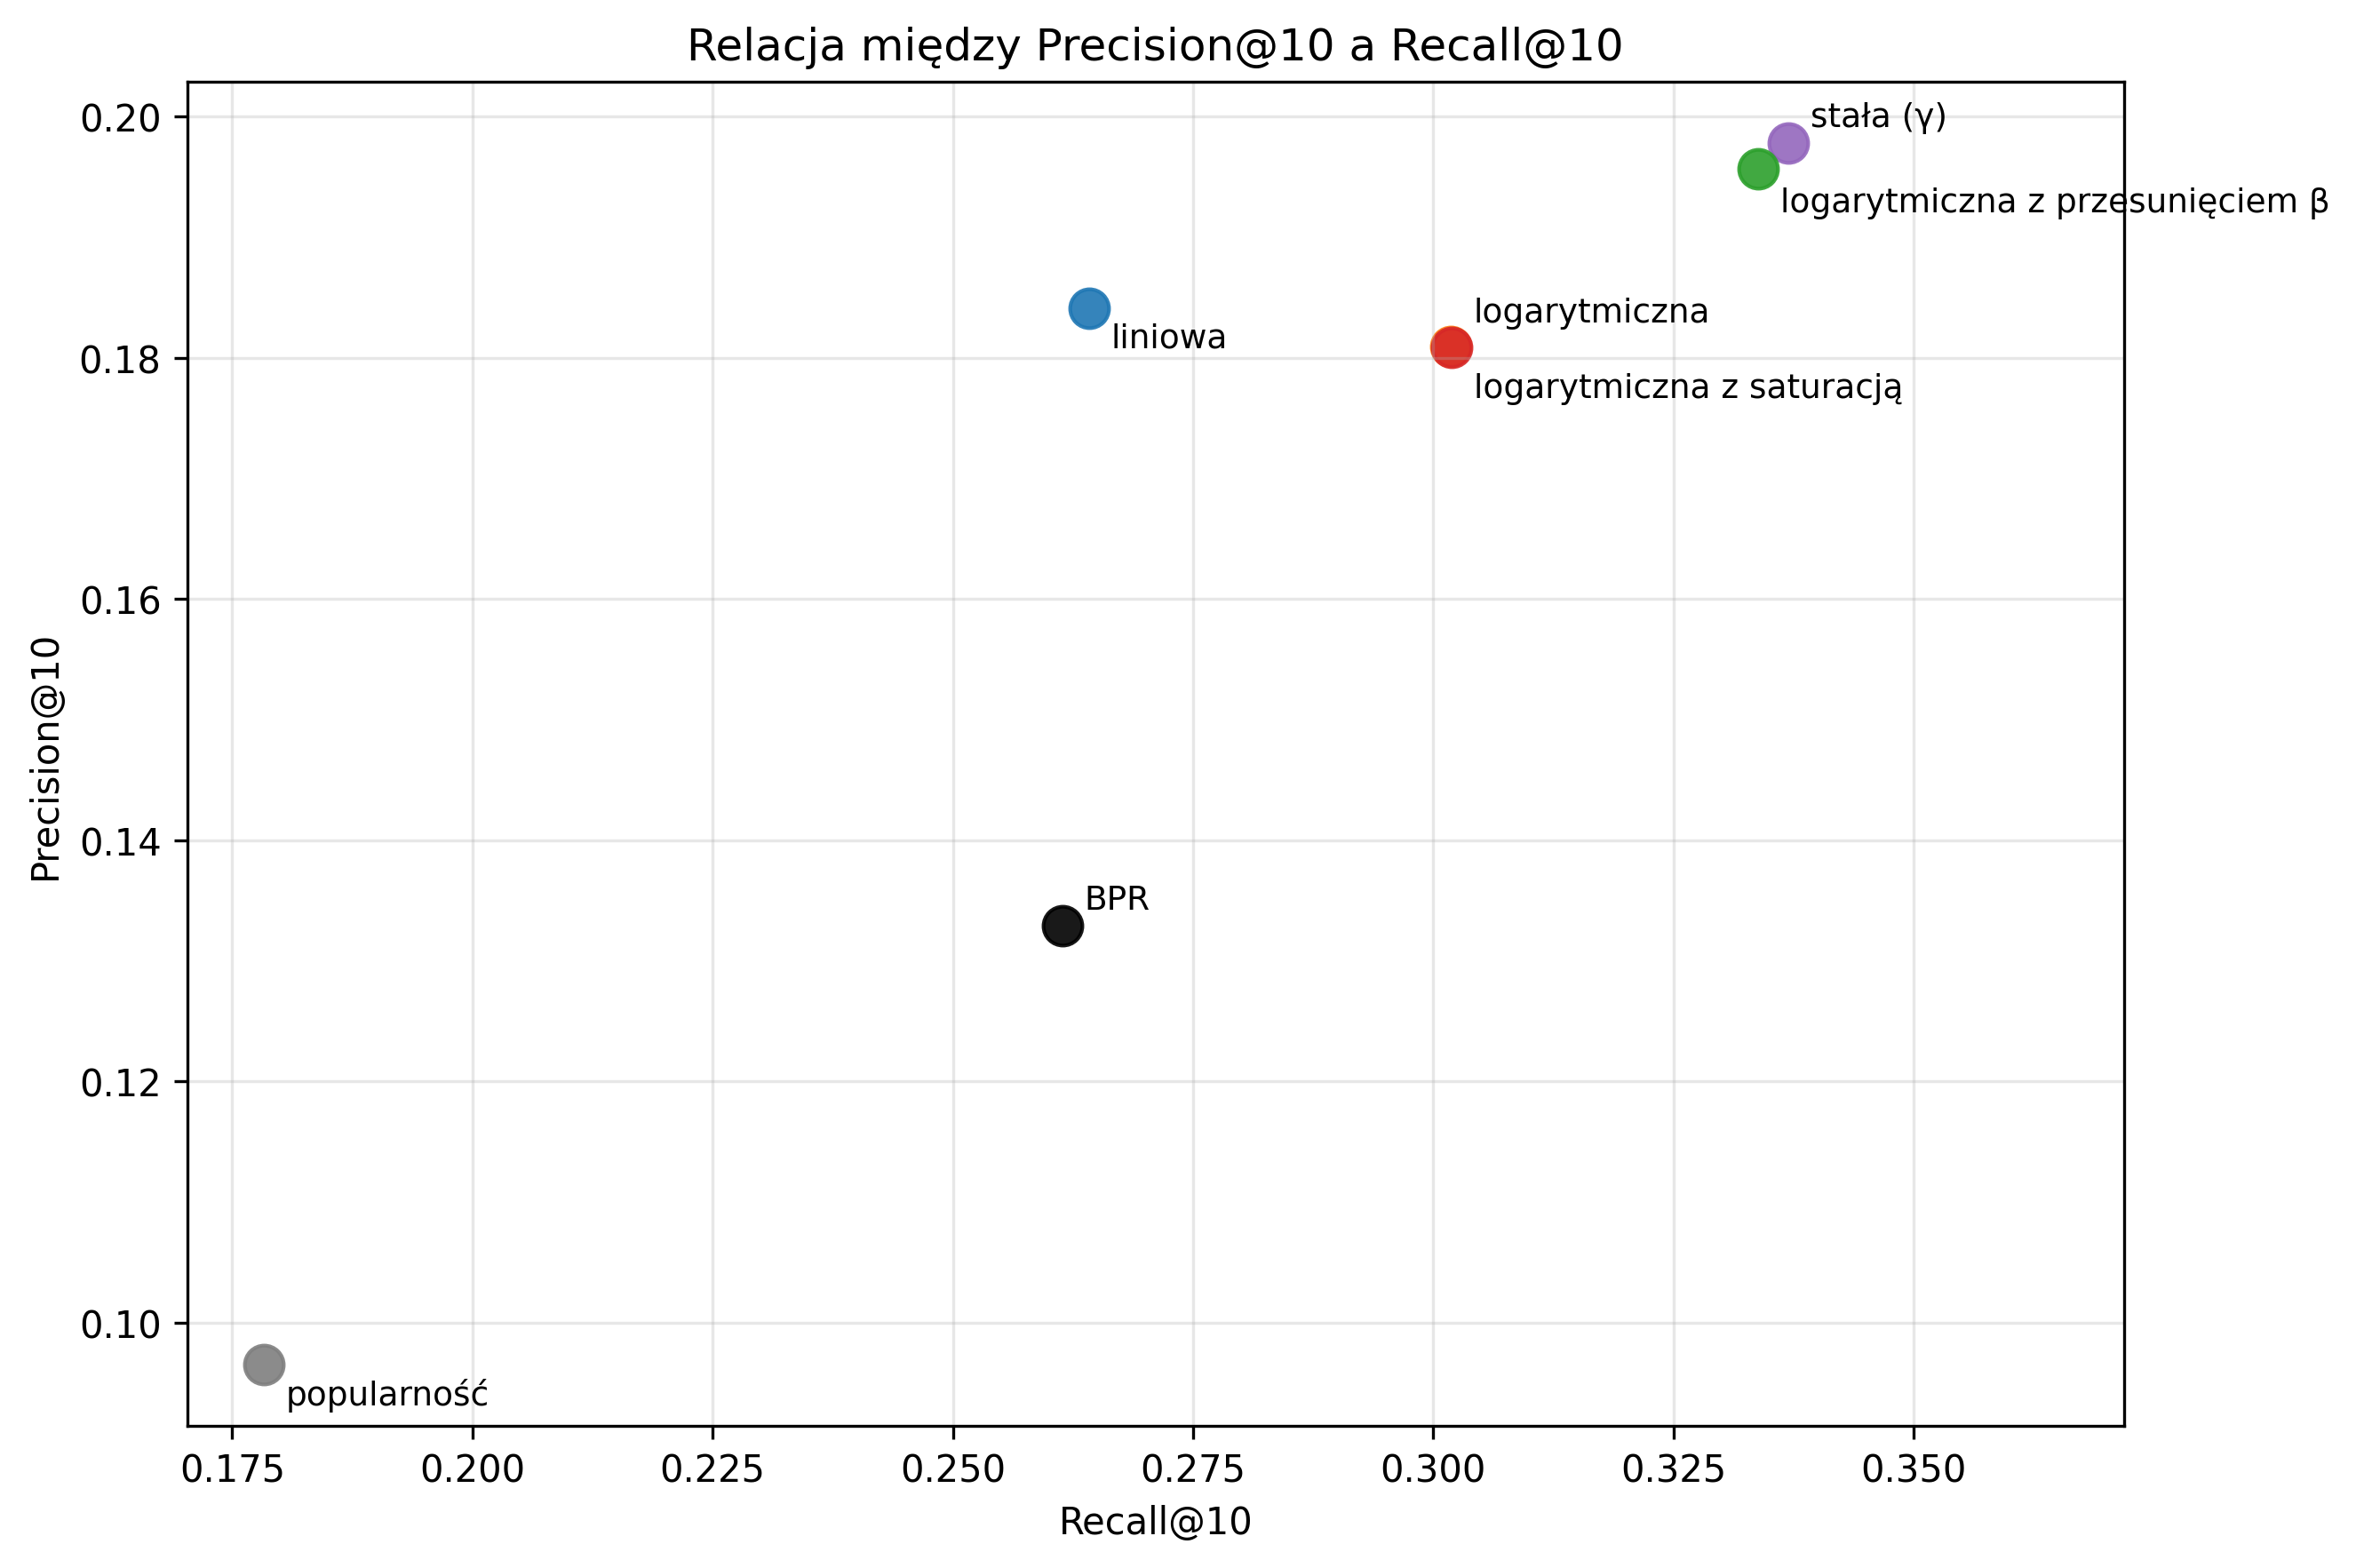
\includegraphics[width=0.9\textwidth]{../results/figures_revised/test_precision_vs_recall_all_models.png}
    \caption{Wartości precyzji względem pełności na zbiorze testowym}
    \label{fig:test_precision_vs_recall_all_models}
\end{figure}

Z wykresu~\ref{fig:test_precision_vs_recall_all_models} można zauważyć, że pomimo niższej wartości metryki pełności od modeli z przekształceniem logarytmicznym i logarytmicznym z saturacją model liniowy ma wyższą wartość precyzji. Może to sugerować, że ten model oferuje trafniejsze rekomendacje w przypadku użytkowników z większą liczbą interakcji. Weryfikacja tej hipotezy wymagałaby podziału użytkowników według liczby posiadanych interakcji, co wykracza poza zakres niniejszej pracy. Widoczne jest również, że warianty o stałej funkcji pewności oraz z przesunięciem $\beta$ wypadają najlepiej w kontekście obu analizowanych metryk, przy czym leżą na wykresie blisko siebie.

\section{Analiza kompromisów jakości rekomendacji}
\label{sec:compromises_analysis}

W procesie ewaluacji systemów rekomendacyjnych istotne jest uwzględnienie również metryk wykraczających poza trafność predykcji (ang. \textit{beyond-accuracy}), takich jak pokrycie katalogu, różnorodność oraz $\Delta$GAP. W niniejszym podrozdziale poddano analizie kompromisy między jakością rekomendacji a wspomnianymi wyżej miarami.

\begin{figure}[htbp]
    \centering
    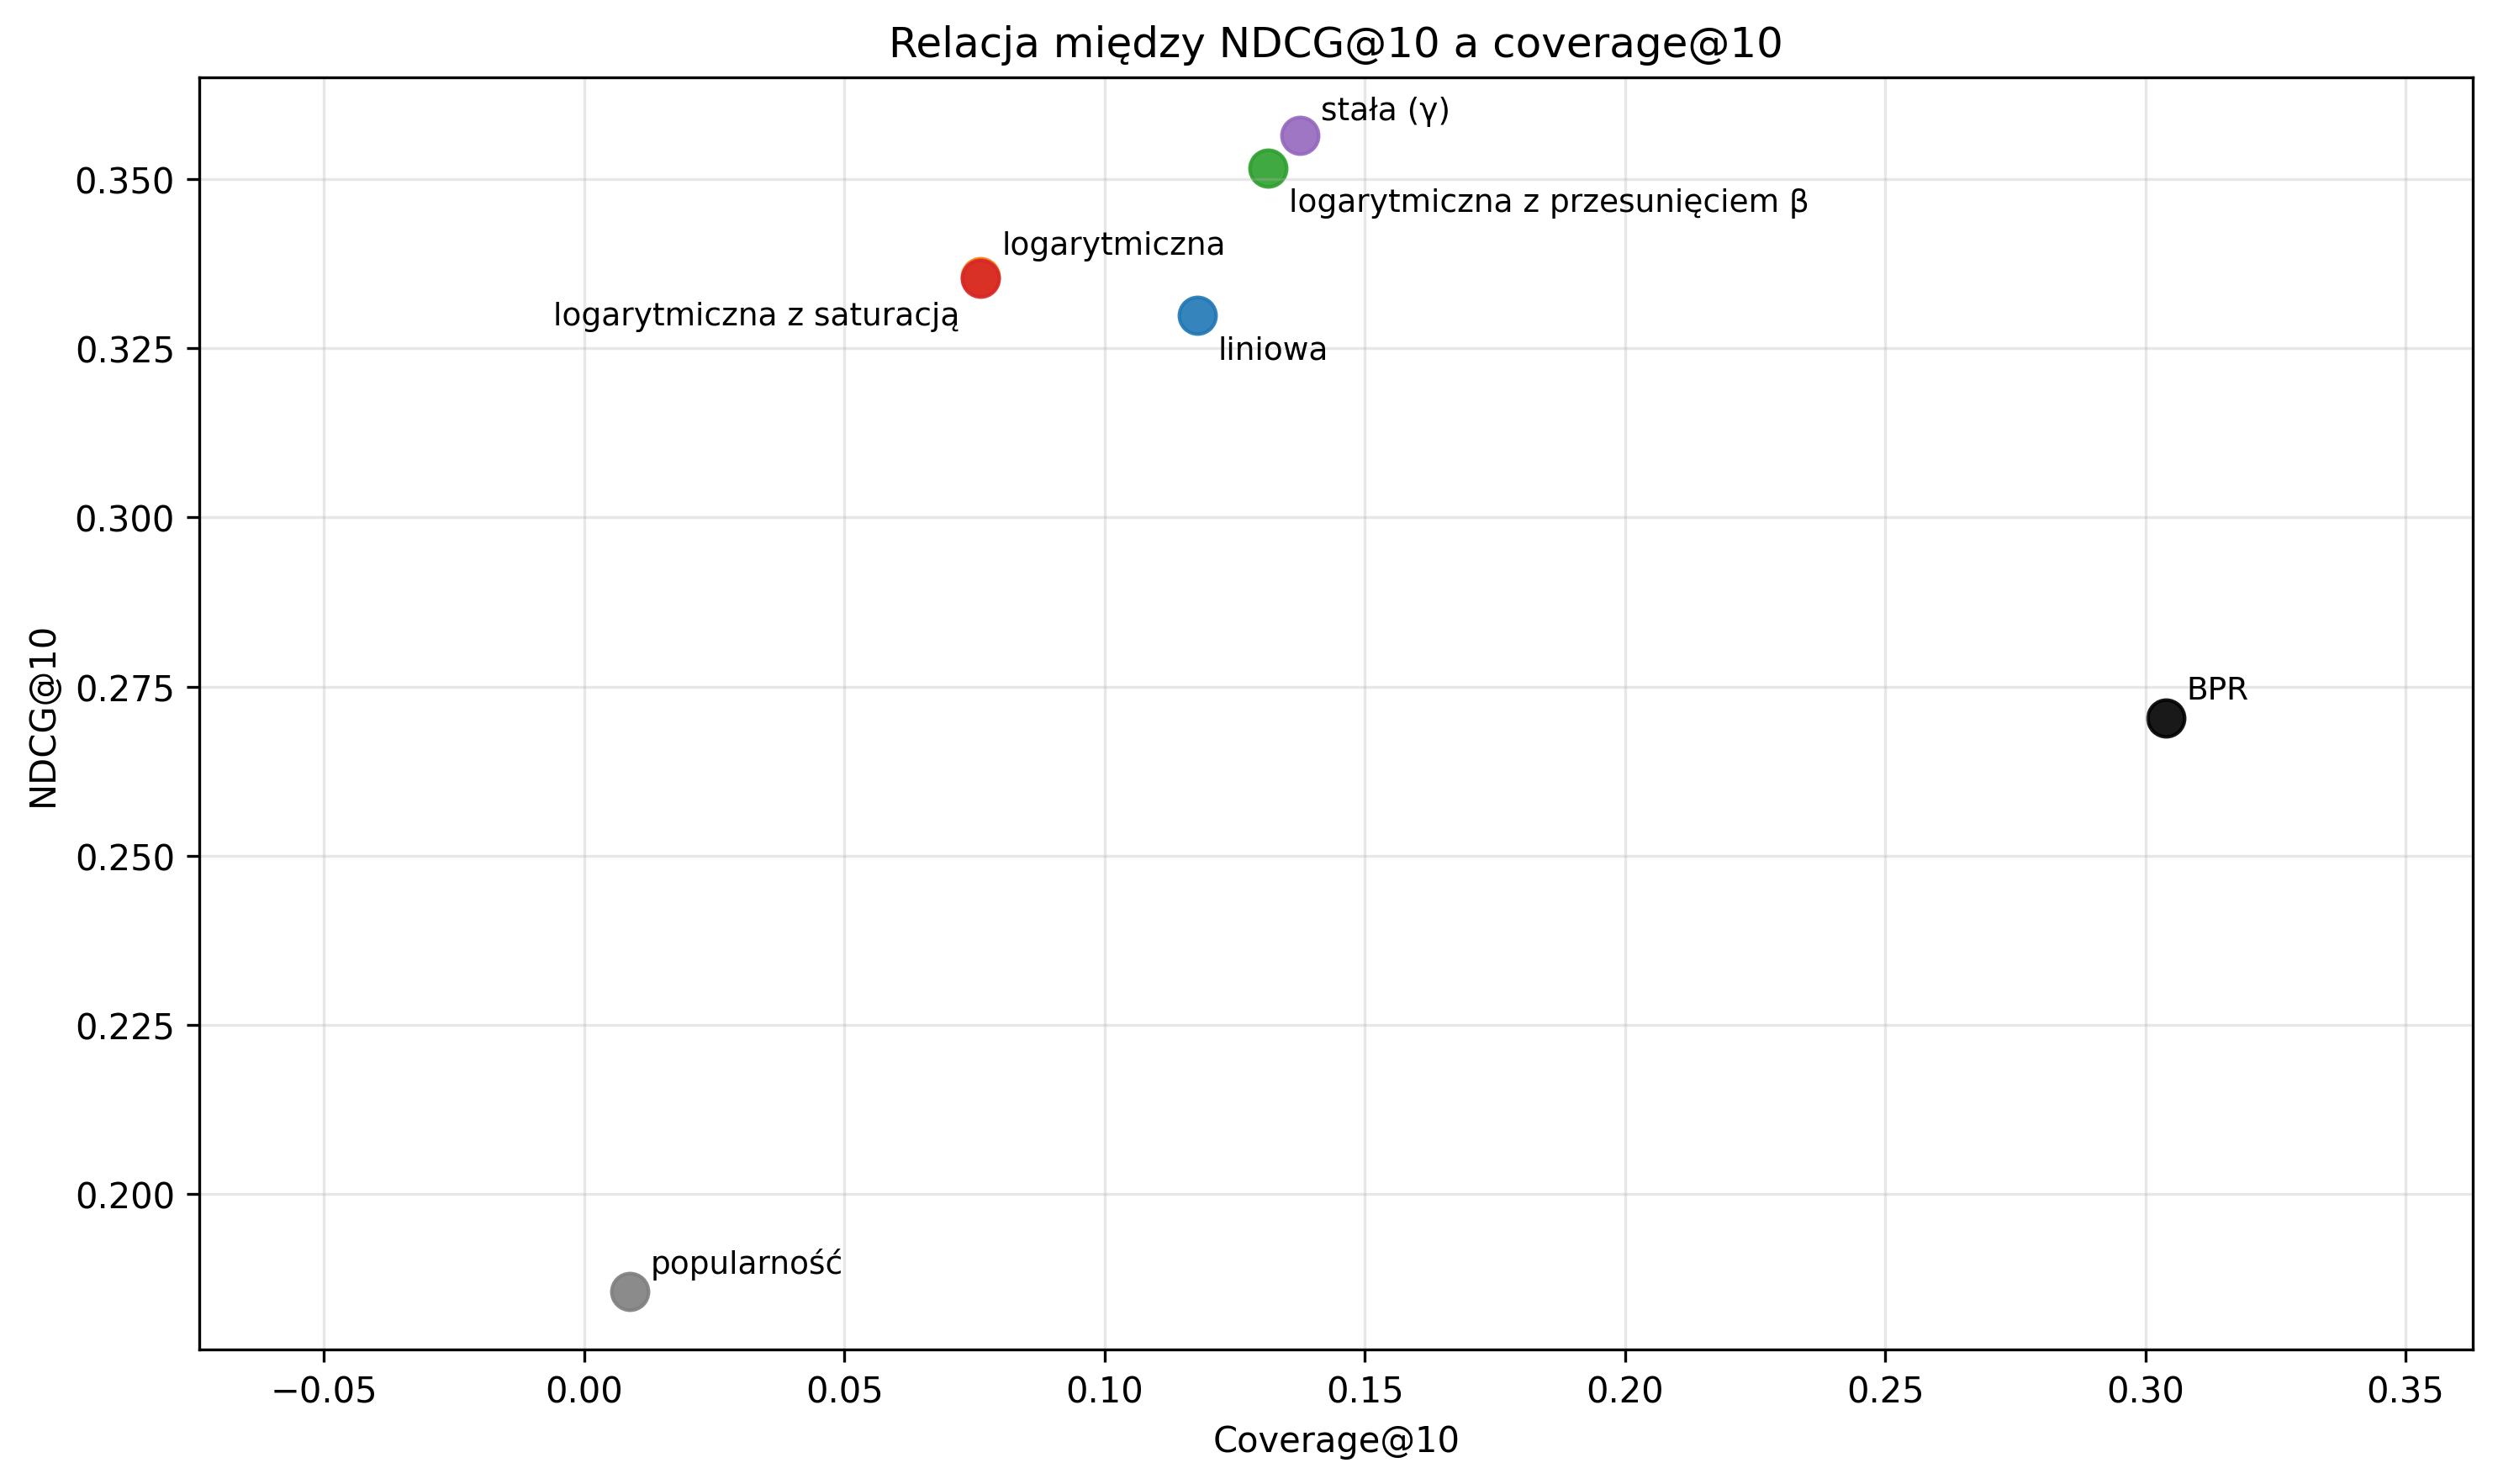
\includegraphics[width=0.9\textwidth]{../results/figures_revised/test_ndcg_vs_coverage_all_models.png}
    \caption{Wartości pokrycia katalogu względem \ndcg{} na zbiorze testowym}
    \label{fig:test_ndcg_vs_coverage_all_models}
\end{figure}

W przypadku metryki pokrycia na wykresie~\ref{fig:test_ndcg_vs_coverage_all_models} widoczna jest znacząca rozbieżność między każdym z badanych typów modeli. Model BPR wykazuje się najwyższym pokryciem (0,3039), będącym ponad dwukrotnie większym niż każdy wariant ALS, jednak osiąga to kosztem niższej wartości \ndcg{}. Rodzina modeli implicit ALS tworzy wyraźne skupienie na wykresie, wewnątrz którego można zaobserwować poprawę wraz ze zwiększeniem bazowej pewności. Najwyższe pokrycie osiąga wariant o stałej funkcji pewności (0,1374), tuż przed wariantem z przesunięciem $\beta$ (0,1313), podczas gdy warianty logarytmiczne pozostają na poziomie około 0{,}076. Oba czołowe warianty wypadają zatem najlepiej pod względem obu przedstawianych metryk, co oznacza, że poprawa jakości rekomendacji nie powstała kosztem faworyzowania wąskiego katalogu obiektów. Niski wynik wariantu popularnościowego pod względem obu metryk jest spójny z oczekiwaniami i wynika z jego niepersonalizowanego charakteru.

Po analizie pokrycia katalogu warto przeanalizować metrykę różnorodności wewnątrzlistowej, opisującą zróżnicowanie pozycji rekomendowanych pojedynczemu użytkownikowi. Miara ta wyznaczana jest na podstawie podobieństwa współwystępowania obiektów w profilach użytkowników w zbiorze treningowym, dzięki czemu pozostaje porównywalna pomiędzy modelami o odmiennych przestrzeniach czynników ukrytych. Model popularnościowy został pominięty w tym porównaniu ze względu na jego niespersonalizowany charakter.

\begin{figure}[htbp]
    \centering
    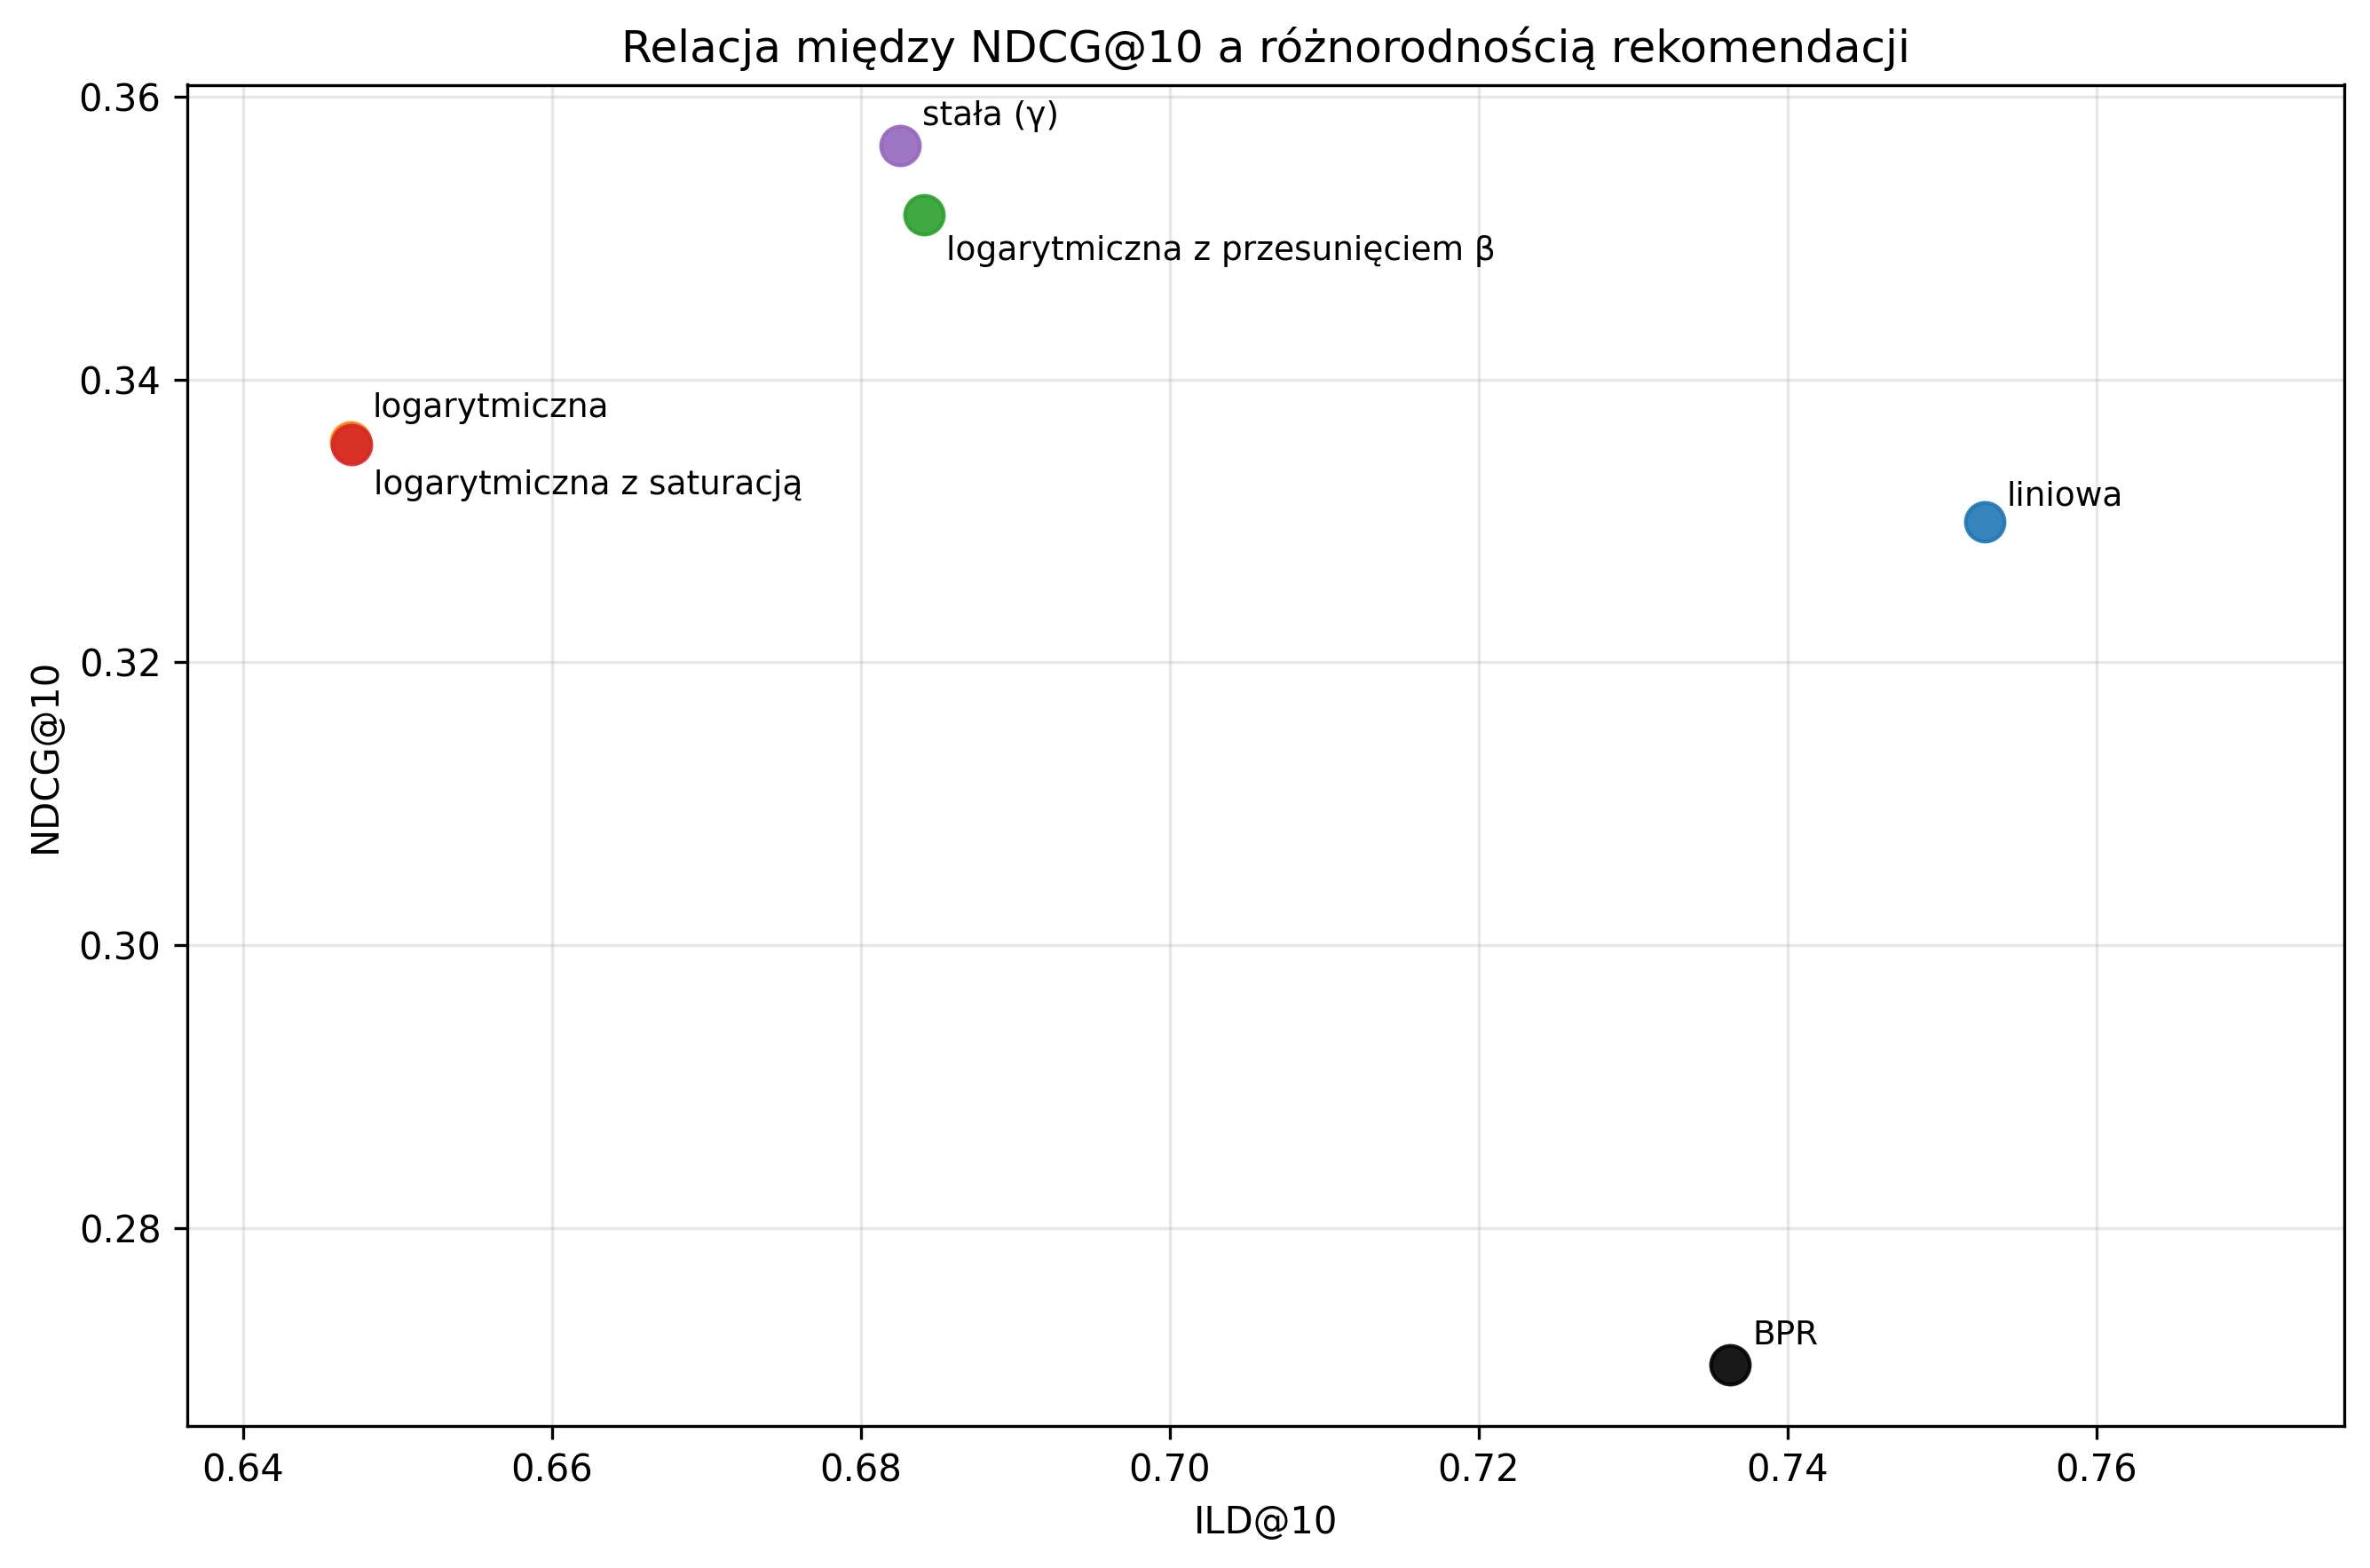
\includegraphics[width=0.9\textwidth]{../results/figures_revised/test_ndcg_vs_ild_cooccurrence.png}
    \caption{Średnie wartości różnorodności wewnątrzlistowej względem \ndcg{} na zbiorze testowym}
    \label{fig:test_ndcg_vs_ild_cooccurrence}
\end{figure}

Na wykresie~\ref{fig:test_ndcg_vs_ild_cooccurrence} zwraca uwagę odrębna pozycja modelu BPR, który przy najniższej wartości \ndcg{} spośród modeli faktoryzacyjnych osiąga wysoką różnorodność (0,7363). W połączeniu z najwyższym pokryciem katalogu wskazuje to, że model ten generuje rekomendacje zarówno silnie zróżnicowane między użytkownikami, jak i wewnątrz jednej listy. Odbywa się to jednak kosztem niższej trafności. Pokazuje to zatem wyraźny kompromis między trafnością a miarami wykraczającymi poza nią.

W obrębie rodziny implicit ALS wartości różnorodności układają się natomiast zgodnie z liczbą czynników ukrytych: warianty logarytmiczne, dysponujące przestrzenią 24-wymiarową, osiągają najniższe wartości (0,6469 oraz 0,6470), warianty stały i z przesunięciem $\beta$ przy 48 czynnikach uzyskują odpowiednio 0,6825 i 0,6841, natomiast wariant liniowy przy 80 czynnikach osiąga wartość najwyższą (0,7528). Warto przy tym zauważyć, że warianty o tej samej wymiarowości uzyskują niemal identyczne wartości, co sugeruje, że wymiar przestrzeni latentnej ma decydujący wpływ na tę metrykę.

Na koniec pozostała do przeanalizowania zależność \ndcg{} od $\Delta\text{GAP}@10$, czyli miary obciążenia rekomendacji popularnością. Wartość zerowa stanowi punkt odniesienia i odpowiada sytuacji, w której popularność rekomendowanych gier jest zbliżona do popularności gier w bibliotece użytkownika zawartych w zbiorze treningowym. Odchylenia w obie strony oznaczają natomiast rekomendowanie pozycji odpowiednio popularniejszych bądź mniej popularnych niż wynikałoby to z profilu użytkownika, przy czym odchylenie w każdą ze stron oznacza rozbieżność z profilem użytkownika. Na wykresie~\ref{fig:test_ndcg_vs_delta_gap_without_popularity} model popularnościowy został ponownie pominięty, aby zachować czytelność pozostałych wyników. Wartość $\Delta\text{GAP}@10$ dla tego modelu wynosi 1,4233, co stanowi maksymalne możliwe obciążenie rekomendacji popularnością w badanym zbiorze.

\begin{figure}[htbp]
    \centering
    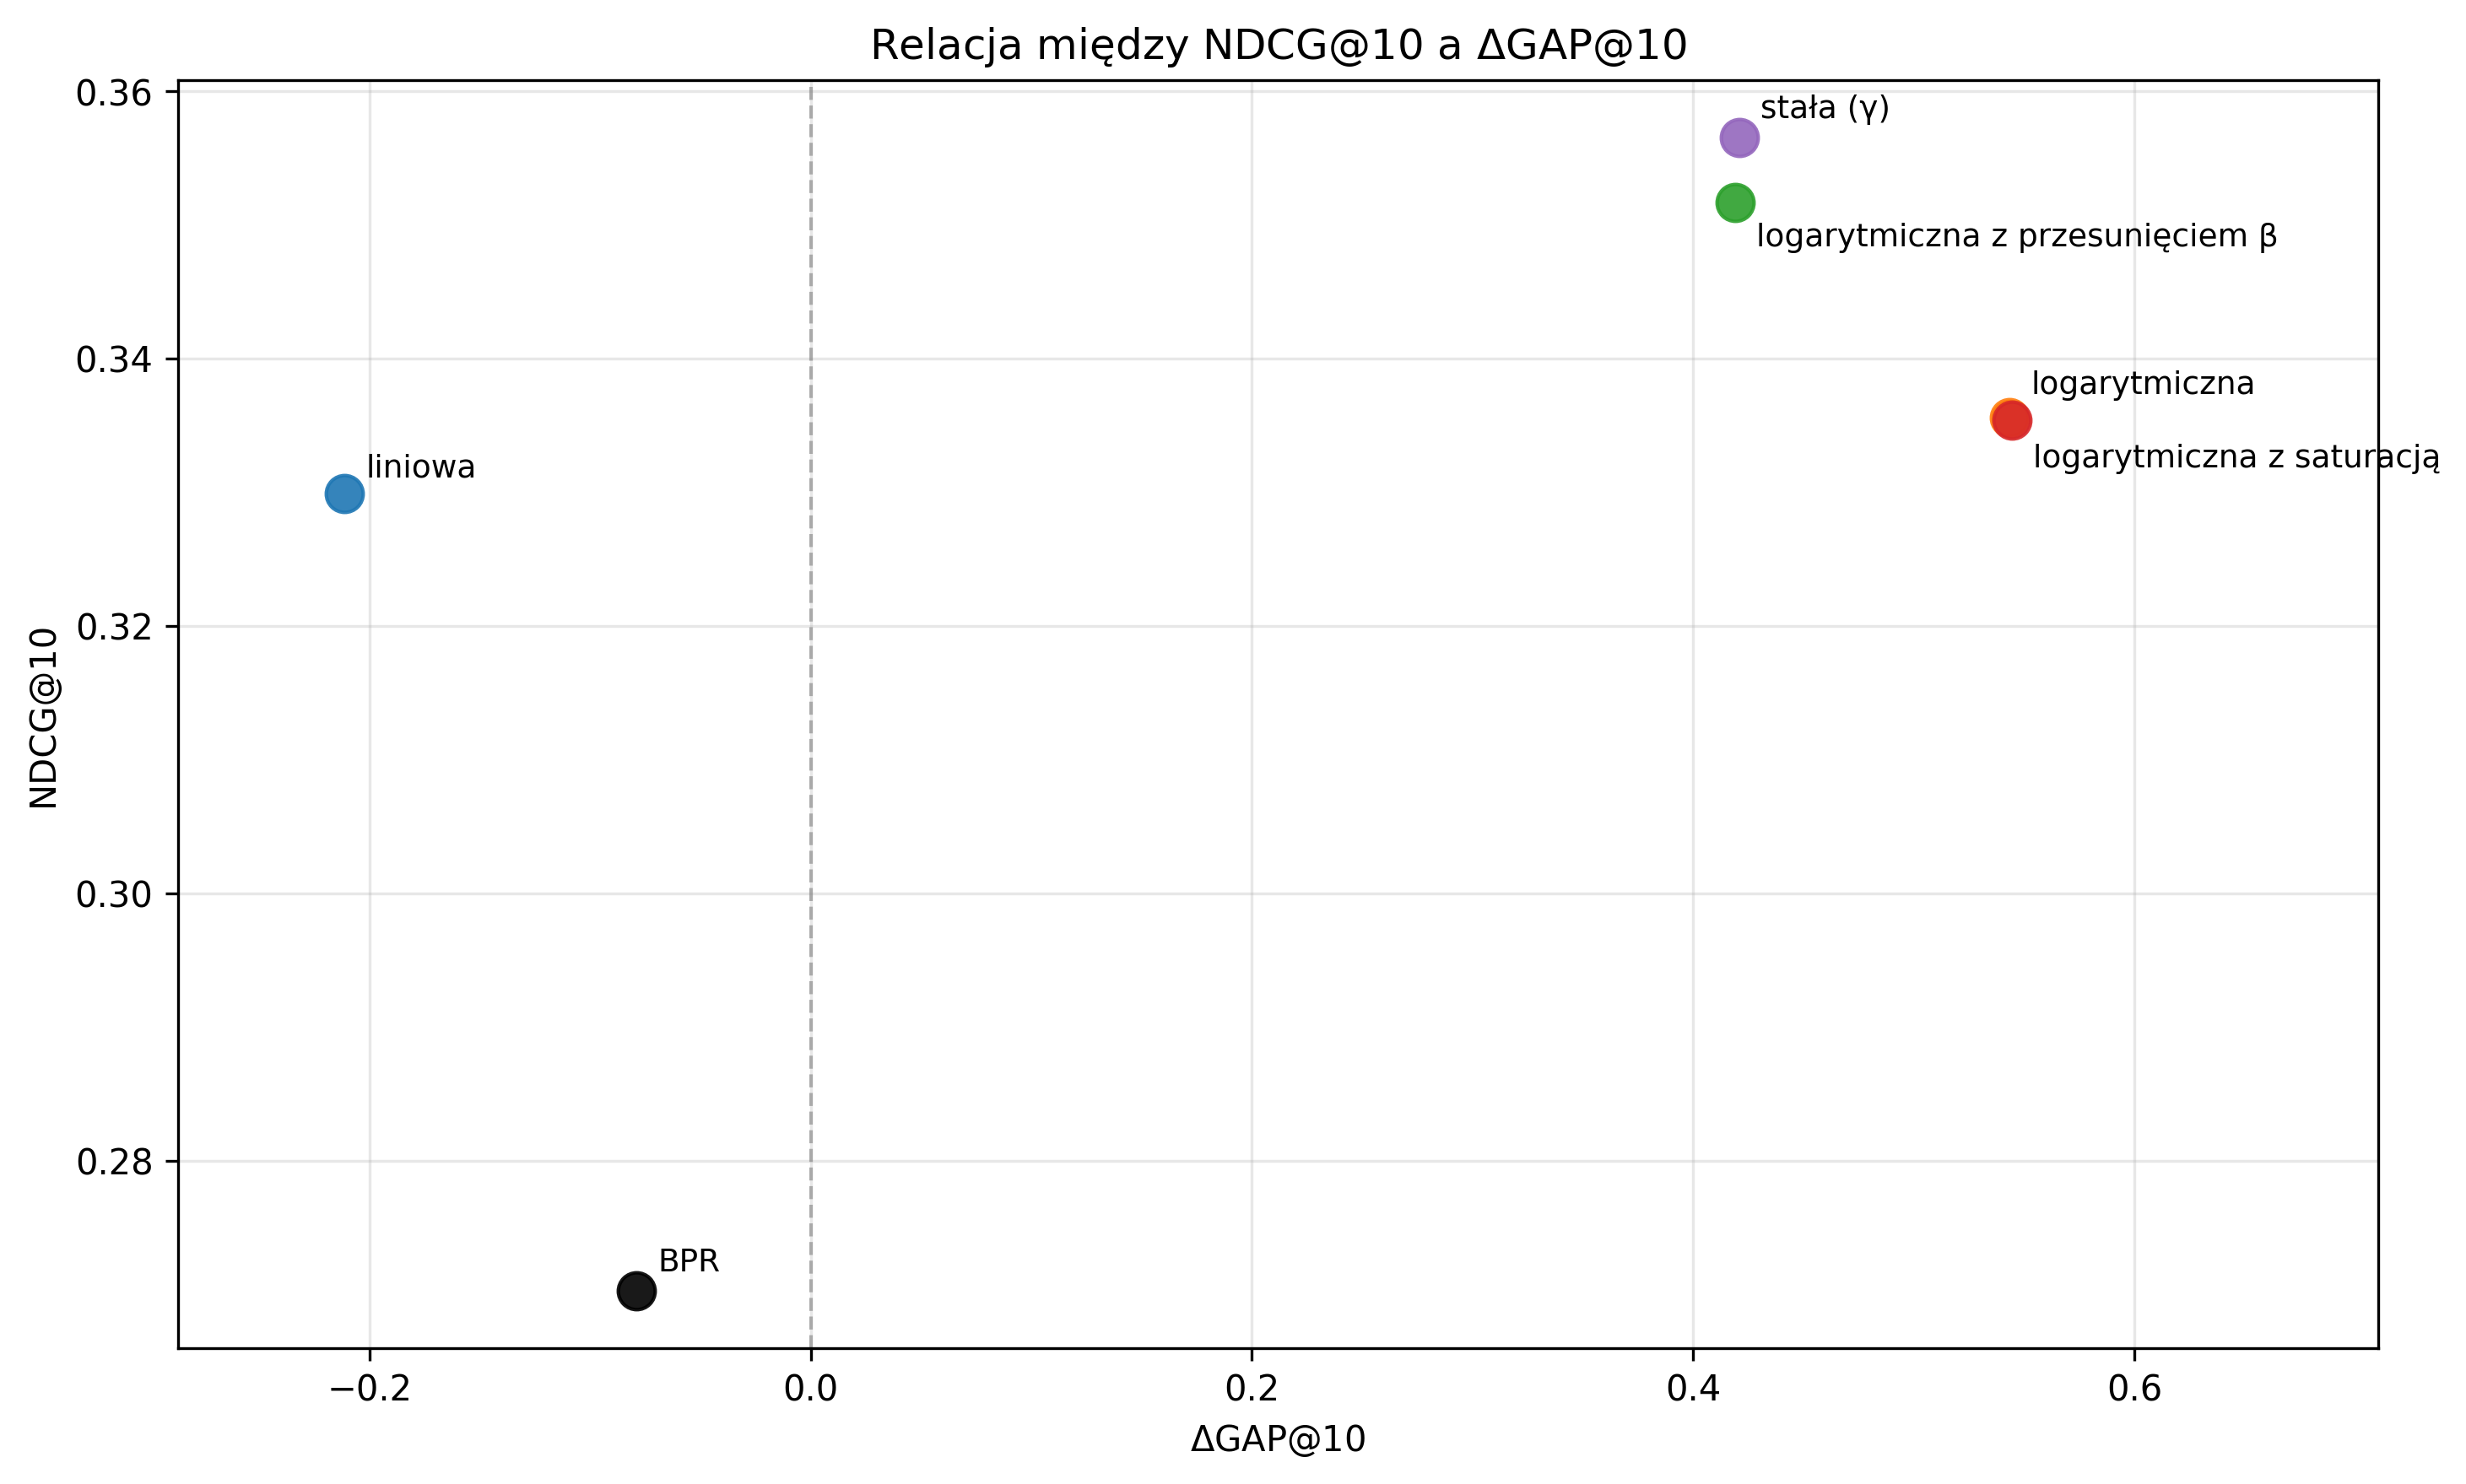
\includegraphics[width=0.9\textwidth]{../results/figures_revised/test_ndcg_vs_delta_gap_without_popularity.png}
    \caption{Średnie wartości $\Delta$GAP względem \ndcg{} na zbiorze testowym}
    \label{fig:test_ndcg_vs_delta_gap_without_popularity}
\end{figure}

Modele BPR oraz implicit ALS z liniową funkcją pewności uzyskały ujemną wartość $\Delta\text{GAP}@10$, co jest nietypowym zachowaniem dla systemów rekomendacyjnych, które mają tendencję do faworyzowania popularnych produktów~\cite{abdollahpouri2019unfairness}. Jednym z~możliwych wyjaśnień jest większa wymiarowość przestrzeni czynników ukrytych obu modeli w~połączeniu ze słabszą regularyzacją. Mniejsza wartość hiperparametrów $\lambda$ oraz $\lambda_\Theta$ dopuszcza wzrost norm wektorów reprezentacji, co umożliwia tworzenie skrajnych dopasowań dla gier o~niskiej popularności. Nie jest to jednak jedyne wyjaśnienie. Ujemna wartość $\Delta\text{GAP}@10$ oznacza odchylenie rekomendacji od profilu użytkownika, które równie dobrze może wynikać ze słabszego dopasowania modelu, a~nie z~trafniejszego rozpoznania preferencji niszowych. Za drugą interpretacją przemawia to, że wariant liniowy osiąga jednocześnie najniższą trafność w~rodzinie implicit ALS. Rozstrzygnięcie między tymi wyjaśnieniami wymagałoby porównania wariantów przy ustalonej liczbie czynników ukrytych, co wykracza poza zakres przeprowadzonego eksperymentu. Wariant liniowy zasługuje przy tym na uwagę, ponieważ łączy ujemną wartość $\Delta\text{GAP}@10$ z największą różnorodnością wewnątrzlistową, jednak traci przy tym na trafności rekomendacji. W przypadku pozostałych modeli ALS ich wartości $\Delta\text{GAP}@10$ są większe od zera, więc rekomendują one gry popularniejsze niż w zbiorze treningowym użytkownika, ale za to cechują się większą trafnością. Na wykresie~\ref{fig:test_ndcg_vs_delta_gap_without_popularity} widać również, że uwzględnienie zwiększonej bazowej wartości pewności nie tylko poprawia trafność rekomendacji, ale również zmniejsza obciążenie popularnością względem wariantów logarytmicznych.

\section{Stabilność wyników}
\label{sec:stabilnosc}

W celu sprawdzenia stabilności wyników obliczono odchylenia standardowe na pięciu uruchomieniach algorytmów implicit ALS i BPR. Wyniki przedstawiono w tabeli~\ref{tab:stabilnosc-zbiorcza}. Metryka ILD@10 została pominięta w analizie stabilności, ponieważ wyznaczono ją dla pojedynczego uruchomienia każdego z modeli.

\begin{table}[htbp]
\centering
\caption{Wyniki na zbiorze testowym wraz z~odchyleniami standardowymi w~pięciu uruchomieniach}
\label{tab:stabilnosc-zbiorcza}
\begin{tabular}{lrrr}
\toprule
Wariant & Precision@10 & Recall@10 & NDCG@10 \\
\midrule
Popularność & $0{,}0965$ & $0{,}1783$ & $0{,}1855$ \\
Liniowa & $0{,}1841\pm0{,}0003$ & $0{,}2642\pm0{,}0005$ & $0{,}3299\pm0{,}0005$ \\
Logarytmiczna & $0{,}1810\pm0{,}0001$ & $0{,}3019\pm0{,}0002$ & $0{,}3356\pm0{,}0003$ \\
Logarytmiczna z saturacją & $0{,}1809\pm0{,}0002$ & $0{,}3019\pm0{,}0003$ & $0{,}3354\pm0{,}0005$ \\
Logarytmiczna z przesunięciem $\beta$ & $0{,}1956\pm0{,}0002$ & $0{,}3338\pm0{,}0003$ & $0{,}3517\pm0{,}0004$ \\
Stała & $0{,}1978\pm0{,}0001$ & $0{,}3370\pm0{,}0002$ & $0{,}3565\pm0{,}0005$ \\
BPR & $0{,}1329\pm0{,}0003$ & $0{,}2614\pm0{,}0005$ & $0{,}2703\pm0{,}0006$ \\
\midrule
Wariant & Coverage@10 & $\Delta$GAP@10 & \\
\midrule
Popularność & $0{,}0087$ & $1{,}4233$ & \\
Liniowa & $0{,}1178\pm0{,}0007$ & $-0{,}2112\pm0{,}0016$ & \\
Logarytmiczna & $0{,}0762\pm0{,}0003$ & $0{,}5433\pm0{,}0008$ & \\
Logarytmiczna z saturacją & $0{,}0761\pm0{,}0002$ & $0{,}5443\pm0{,}0009$ & \\
Logarytmiczna z przesunięciem $\beta$ & $0{,}1313\pm0{,}0009$ & $0{,}4191\pm0{,}0023$ & \\
Stała & $0{,}1374\pm0{,}0004$ & $0{,}4210\pm0{,}0008$ & \\
BPR & $0{,}3039\pm0{,}0012$ & $-0{,}0789\pm0{,}0054$ & \\
\bottomrule
\end{tabular}
\caption*{\footnotesize Wartości dla modeli implicit ALS oraz BPR stanowią średnie z~pięciu uruchomień o~różnym ziarnie inicjalizacji. Model popularnościowy jest deterministyczny, dlatego podano dla niego pojedynczy wynik. Źródło: opracowanie własne.}
\end{table}

Analiza odchyleń standardowych uzyskanych w pięciu losowych inicjalizacjach algorytmów implicit ALS i BPR potwierdza wysoką stabilność wszystkich badanych modeli. W przypadku metryk trafności rekomendacji odchylenia standardowe nie przekraczają $0{,}0006$, co odpowiada mniej niż $0{,}2\%$ wartości średniej. Świadczy to o tym, że przedstawione różnice jakościowe między modelami nie wynikają z losowości inicjalizacji. Z kolei najwyższe odchylenie względne zaobserwowano przy metryce $\Delta$GAP@10 dla modelu BPR, które wynosi $6{,}84\%$ przy wartości średniej równej $-0{,}0789$. Ze względu na znikome różnice wynikające z odchyleń wykresy mające na celu je przedstawić zostały pominięte.

\begin{table}[htbp]
\centering
\caption{Wyniki na zbiorze walidacyjnym wraz z~odchyleniami standardowymi w~pięciu losowych podziałach danych}
\label{tab:stabilnosc-walidacja-zbiorcza}
\begin{tabular}{lrrr}
\toprule
Wariant & Precision@10 & Recall@10 & NDCG@10 \\
\midrule
Popularność & $0{,}0811\pm0{,}0002$ & $0{,}1719\pm0{,}0002$ & $0{,}1615\pm0{,}0004$ \\
Liniowa & $0{,}1360\pm0{,}0006$ & $0{,}2302\pm0{,}0008$ & $0{,}2466\pm0{,}0011$ \\
Logarytmiczna & $0{,}1349\pm0{,}0009$ & $0{,}2589\pm0{,}0019$ & $0{,}2534\pm0{,}0018$ \\
Logarytmiczna z saturacją & $0{,}1350\pm0{,}0008$ & $0{,}2596\pm0{,}0015$ & $0{,}2536\pm0{,}0015$ \\
Logarytmiczna z przesunięciem $\beta$ & $0{,}1479\pm0{,}0005$ & $0{,}2963\pm0{,}0012$ & $0{,}2744\pm0{,}0011$ \\
Stała & $0{,}1502\pm0{,}0003$ & $0{,}3007\pm0{,}0010$ & $0{,}2792\pm0{,}0007$ \\
\midrule
Wariant & Coverage@10 & $\Delta$GAP@10 & \\
\midrule
Popularność & $0{,}0069\pm0{,}0002$ & $1{,}5138\pm0{,}0011$ & \\
Liniowa & $0{,}1025\pm0{,}0003$ & $-0{,}2048\pm0{,}0010$ & \\
Logarytmiczna & $0{,}0636\pm0{,}0006$ & $0{,}4899\pm0{,}0071$ & \\
Logarytmiczna z saturacją & $0{,}0635\pm0{,}0006$ & $0{,}4942\pm0{,}0047$ & \\
Logarytmiczna z przesunięciem $\beta$ & $0{,}1138\pm0{,}0017$ & $0{,}4072\pm0{,}0119$ & \\
Stała & $0{,}1208\pm0{,}0006$ & $0{,}4256\pm0{,}0079$ & \\
\bottomrule
\end{tabular}
\caption*{\footnotesize Analizę przeprowadzono na pięciu losowych podziałach na zbiór treningowy i~walidacyjny przy ustalonym ziarnie inicjalizacji modelu. Źródło: opracowanie własne.}
\end{table}

W związku z zastosowaniem wydzielonego zbioru testowego zamiast procedury walidacji krzyżowej przeprowadzono analizę stabilności względem losowego podziału danych. W tabeli~\ref{tab:stabilnosc-walidacja-zbiorcza} przedstawiono wartości średnie metryk oraz odchylenia standardowe liczone na pięciu losowych podziałach na zbiory treningowe i walidacyjne. Analizę tę ograniczono do modeli implicit ALS oraz modelu popularnościowego. Największą względną wartość odchylenia standardowego odnotowano dla metryki $\Delta$GAP@10 w~wariancie logarytmicznym z~przesunięciem $\beta$, gdzie wynosi ona $2{,}92\%$. Tak niski poziom zmienności wynika najprawdopodobniej ze znacznego rozmiaru wykorzystanego zbioru danych, który uodparnia proces uczenia na~różnice wynikające z~losowego podziału. Ze względu na niewielką skalę odchyleń zrezygnowano z~ich graficznej prezentacji.

\section{Odniesienie wyników do literatury}
\label{sec:porownanie-literatura}

Ograniczona porównywalność i~odtwarzalność wyników stanowi rozpoznany problem w~dziedzinie systemów rekomendacyjnych~\cite{dacrema2019progress}. Z~tego powodu przedstawione rezultaty należy traktować jako zamknięty eksperyment, w~którym wszystkie modele oceniano na tym samym zbiorze, przy identycznej procedurze filtracji, podziału danych oraz ewaluacji. Uzyskane wyniki pozwalają zatem przede wszystkim na porównanie badanych wariantów między sobą w~ramach przyjętej metodologii. Podjęto jednak próbę odniesienia uzyskanych wyników do prac wykorzystujących ten sam zbiór danych.

W~celu weryfikacji poprawności zaimplementowanego procesu trenowania modeli odtworzono wyniki przedstawione w~opracowaniu Bayrama~\cite{bayram2021game}. Stosowana tam metryka, określana przez autora jako Precision@10, odpowiadająca w~praktyce mierze HitRate@10, wyznaczającej odsetek użytkowników, dla których ukryta interakcja znalazła się wśród dziesięciu pierwszych pozycji rankingu. Raportowana wartość wynosi 31,60\%, natomiast w~replikacji uzyskano 29,18\%. Zbieżność obu wyników potwierdza poprawność przyjętej implementacji, a~pozostała różnica wynika przypuszczalnie z~nie w~pełni odtworzonego przygotowania danych, obejmującego między innymi wykorzystanie dodatkowych zbiorów udostępnianych dla platformy Steam. Należy przy tym podkreślić, że w~odtwarzanej pracy zastosowano ewaluację metodą leave-one-out z~próbkowaniem negatywnym, przez co replikacja pełni funkcję kontroli poprawności procesu modelowania, nie zaś punktu odniesienia dla wyników przedstawionych w~niniejszym rozdziale.

Pozostałe badania wykorzystujące dane platformy Steam, do których odnoszono się w~pracy, różnią się od niej w~stopniu uniemożliwiającym zestawienie wartości metryk. Bunga i~in.~\cite{bunga2021implicit} przekształcają czas gry w~ocenę, sprowadzając zadanie do predykcji jawnych ocen, a~ponadto usuwają interakcje z~zerowym czasem gry, użytkowników posiadających mniej niż 30 gier oraz gry występujące u~mniej niż 10 użytkowników. Cheuque i~in.~\cite{cheuque2019steam} koncentrują się natomiast na modelach neuronowych, stosując walidację krzyżową oraz wyraźnie silniejszą filtrację danych. W~obu przypadkach zabiegi te prowadzą do innego zadania ewaluacyjnego niż rozważane w~niniejszej pracy, co znajduje odzwierciedlenie w~różnicach między wartościami raportowanych metryk.